% \iffalse meta-comment ^^A 此行的\iffalse 和 \end{document}后的那个\fi配对,用以在获得说明文档时越过.ins 文件
% !TeX program  = XeLaTeX
% !TeX encoding = UTF-8%
%
% cexam.dtx
% Copyright 2016-2019 FengZhenhua <fengzhenhua@sina.cn>
% 
% 此版本是为了适应latex3,以便更好的维护系统,于2019年4月9日晚决定在空闲时间将已经由latex2e开发完成的cexam.sty,使用latex3改写全部代码.2019年9月3日,经过近一周的奋斗,成功构建成了v3.1.3版本,它初步实现了选择,填空,判断,计算四种题型的自动排版.接下来的一段时间内,不做重大功能上的增加,停留一段时间,用来检验和优化代码.
%
% 由于立志通过北京大学的理论物理考试,同时工作又需要消耗大量的时间,一边学习一边工作一边搞 \pkg{cexam} 的开发,这很紧张.所以决定以考研大业为主,工作其次, \pkg{cexam} 改写工作于空闲时间进行.祝自己成功!!
%
% 2019年9月10在紧张的学习过程中,依然抽出了一天的时间做了一个版本上的优化.精简了一些长度付值的命令,优化了排版逻辑结构,效率更加高效.同时对于矩形生成程序加入了专有宽度,不与其它程序共用,这样做的优点是程序更加稳定.
% 
% 2019年9月18日在上完今天的课后,完成了学生答案模式写出功能的添加,同时支持答案的超链接生成标签.版本号为v3.1.6 ,此版本基本完成了试题排版的工作,所以它是一个可用的版本,之后会优化一些现有代码为主,等到更加高效稳定生考虑加入其它功能.
%
% 
% 2019年 09月 19日 星期四 18:54:01 CST 今天去除了一些bug,同时加入了例题模式.版本号为v3.1.7,可以应用于工作环境中.
% 2020年 03月 28日 星期六 14:46:13 CST 修改完成大部分使用\LaTeXiii{}命令改写的代码,版本号v3.2.6。在生成文档时,确定版本的\cs{GetIdInfo}是在宏包中确定的,所以在生成宏包后用新的宏包编译才可以生成对应的文档。
% 
%<*internal>
\iffalse
%</internal>
%
%<*readme>
cexam
=====

`cexam` is a macro package for  Chinese middle school examination.

Authors and Contributors
------------------------
* Feng Zhenhua <fengzhenhua@sina.cn>

Contributing
------------
This package was created by Feng Zhenhua.

Copyright and Licence
---------------------
    Copyright (C) 2017--2020
    FengZhenhua and any individual authors listed elsewhere in this file.
    ----------------------------------------------------------------------

    This work may be distributed and/or modified under the
    conditions of the LaTeX Project Public License, either
    version 1.3c of this license or (at your option) any later
    version. This version of this license is in
       http://www.latex-project.org/lppl/lppl-1-3c.txt
    and the latest version of this license is in
       http://www.latex-project.org/lppl.txt
    and version 1.3 or later is part of all distributions of
    LaTeX version 2005/12/01 or later.

    This work has the LPPL maintenance status `maintained'.

    The Current Maintainers of this work is Feng Zhenhua.

    This package consists of the file cexam.dtx
                and the derived files cexam.sty
				      README.md (this file).
  ------------------------------------------------------------------------------
%</readme>
%
%<*internal>
\fi
%</internal>
%
%<*internal>
\begingroup
  \def\temp{LaTeX2e}
\expandafter\endgroup\ifx\temp\fmtname\else 
\csname fi\endcsname
%</internal>
%
%<*install>
\input ctxdocstrip %
\askforoverwritefalse
\keepsilent

\preamble

    Copyright (C) 2017--2020
    Feng Zhenhua and any individual authors listed elsewhere in this file.
    ----------------------------------------------------------------------

    This work may be distributed and/or modified under the
    conditions of the LaTeX Project Public License, either
    version 1.3c of this license or (at your option) any later
    version. This version of this license is in
       http://www.latex-project.org/lppl/lppl-1-3c.txt
    and the latest version of this license is in
       http://www.latex-project.org/lppl.txt
    and version 1.3 or later is part of all distributions of
    LaTeX version 2005/12/01 or later.

    This work has the LPPL maintenance status `maintained'.

    The Current Maintainers of this work is Feng Zhenhua.

------------------------------------------------------------------------------
\endpreamble
%
\postamble
\endpostamble
%
\generate 
{
    \usedir{tex/latex/cexam}
    \file{cexam.sty}	            {\from{\jobname.dtx}{package}}
%</install>
%<*internal>
    \usedir{source/latex/cexam}
    \file{\jobname.ins}                    {\from{\jobname.dtx}{install}}
%</internal>
%<*install>
    \nopreamble\nopostamble
    \usedir{doc/latex/cexam}
    \file{README.md}                {\from{\jobname.dtx}{readme}}
}

\catcode32=12\space

\Msg{*************************************************************}
\Msg{                                                             }
\Msg{ To finish the installation you have to move the following   }
\Msg{ file into proper directories searched by TeX:               }
\Msg{                                                             }
\Msg{  cexam.sty and cexam.pdf                                    }
\Msg{                                                             }
\Msg{ The recommended directory is TDS:                           }
\Msg{                                                             }
\Msg{/usr/local/texlive/texmf-local/tex/latex/local/cexam.sty      }
\Msg{                                                             }
\Msg{/usr/local/texlive/texmf-local/doc/local/cexam.pdf            }
\Msg{								  }
\Msg{ To produce the documentation run the file cexam.dtx	  }
\Msg{ through XeLaTeX.						  }
\Msg{								  }
\Msg{ Happy TeXing!						  }
\Msg{								  }
\Msg{*************************************************************}

\endbatchfile 
%</install>
%<*internal>
\fi  
%</internal>
%
%<package>\NeedsTeXFormat{LaTeX2e}
%<package>\RequirePackage{expl3,l3keys2e,xparse,l3draw}
%<package>\GetIdInfo$Id: cexam.dtx v3.2.8(testing)  2020-07-14  ZhenhuaFeng  <fengzhenhua@sina.cn> $ {For Chinese middle school examination}
%<package>\ProvidesExplPackage{\ExplFileName}{\ExplFileDate}{\ExplFileVersion}{\ExplFileDescription}
%
%<*driver>
\documentclass{ctxdoc}
\usepackage[user=teacher]{cexam} ^^A 引入宏包,用以生成说明文档,展示排版效果
\usepackage{tikz}
\EnableCrossrefs
\CodelineIndex
\RecordChanges
%\OnlyDescription
\begin{document}
  \DocInput{\jobname.dtx}
  \IndexLayout
  \PrintChanges
  \PrintIndex
\end{document}
%</driver>
%
% \fi ^^A 此\fi 和第1行的\iffalse 配对
% 
% \changes{v3.0.0}{2019/04/09}{开始使用 \LaTeXiii{}重构cexam.sty}
% \changes{v3.0.1}{2019/07/31}{加入测行程序和形状生成程序,同时删除之前改写的代码}
% \changes{v3.0.1}{2019/07/31}{缩写命名,加入缩写列表}
% \changes{v3.0.7}{2019/08/15}{删除命令\cs{cexam_stand_dim:n}}
% \changes{v3.0.7}{2019/08/15}{删除命令\cs{cexam_fmt_pic:n}}
% \changes{v3.1.0}{2019/08/25}{引入宏包xcolor}
% \changes{v3.1.2}{2019/08/29}{重新改写测行程序}
% \changes{v3.1.2}{2019/08/29}{删除了一些旧的代码}
% \changes{v3.1.3}{2019/09/03}{selection更名为choice}
% \changes{v3.1.3}{2019/09/03}{对cexam.dtx文件,修改了版权信息}
% \changes{v3.1.4}{2019/09/10}{进行了程序精简,更加稳定}
% \changes{v3.1.4}{2019/09/10}{删除了长度命令\cs{cexam_fmtwd_dim}}
% \changes{v3.1.6}{2019/09/18}{加入答案写出功能}
% \changes{v3.1.6}{2019/09/18}{答案支持超链接}
% \changes{v3.1.6}{2019/09/18}{修改了文档中的一些输入文本错误}
% \changes{v3.1.7}{2019/09/19}{增加例题模式}
% \changes{v3.1.7}{2019/09/21}{引入宏包tikz}
% \changes{v3.1.8}{2019/09/22}{增加源文档中的一些命令解释和题目输入举例}
% \changes{v3.1.9}{2019/09/29}{优化了说明档,增加题型排版展示和安装说明}
% \changes{v3.2.2}{2019/02/16}{此版主要的工作是规范了\LaTeXiii{}格式,替换原来的一些命令为字符串变量}
% \changes{v3.2.2}{2019/02/16}{删除\cs{sep_hd_old:},\cs{sp_hd_old_add:n}}
% \changes{v3.2.3}{2020/03/21}{去除宏包\pkg{xcolor},\pkg{tikz}}
% \changes{v3.2.4}{2020/03/22}{删除\cs{cexam_pic_det:n},去除宏包\pkg{calc}}
% \changes{v3.2.5}{2020/03/27}{删除测行程序之外的\cs{parbox}命令}
% \changes{v3.2.6}{2020/03/28}{以\cs{c_empty_tl}取代\cs{relax}}
% \changes{v3.2.6}{2020/04/19}{修改宏包的安装路径为默认路径}
% \changes{v3.2.7}{2020/07/12}{删除\cs{ind_hat_hdim}}
% \changes{v3.2.8}{2020/07/14}{增加证明题环境,但是在一般文档中启用学生模式会出现错误,在下一版中修复}
%
%
% \CheckSum{0}
%
% \CharacterTable
%  {Upper-case    \A\B\C\D\E\F\G\H\I\J\K\L\M\N\O\P\Q\R\S\T\U\V\W\X\Y\Z
%   Lower-case    \a\b\c\d\e\f\g\h\i\j\k\l\m\n\o\p\q\r\s\t\u\v\w\x\y\z
%   Digits        \0\1\2\3\4\5\6\7\8\9
%   Exclamation   \!     Double quote  \"     Hash (number) \#
%   Dollar        \$     Percent       \%     Ampersand     \&
%   Acute accent  \'     Left paren    \(     Right paren   \)
%   Asterisk      \*     Plus          \+     Comma         \,
%   Minus         \-     Point         \.     Solidus       \/
%   Colon         \:     Semicolon     \;     Less than     \<
%   Equals        \=     Greater than  \>     Question mark \?
%   Commercial at \@     Left bracket  \[     Backslash     \\
%   Right bracket \]     Circumflex    \^     Underscore    \_
%   Grave accent  \`     Left brace    \{     Vertical bar  \|
%   Right brace   \}     Tilde         \~}
%
% \title{中文试题排版 cexam 宏包手册}
% \author{冯振华}
% \date{\ExplFileDate\qquad\ExplFileVersion\thanks{fengzhenhua@sina.cn}}
% \maketitle
%
% 
% \begin{abstract}
% 我是一名高中物理教师,所以在工作中不可避免的会遇到输入数学公式的问题,同时我也希望能够将自己多年的备课及解决的疑难问题记录下来,以备学生们在复习时或者刚开始学习物理的同学作为教材的补充使用.历经各种困难,最后找到了\LaTeX{},发现了这个举世无双的神奇软件.2016年自学了一年的宏包编写,成功解决了高中的物理数学试卷的排版问题。但是之前直接写的sty文件和cls文件,实现了选择、填空、计算等题型的自动排版,同时实现批量处理各种题型、实现数学与图片的排版、自动生成beamer文档、生成答题卡、教师与学生不同模式排版。但是后来发现,功能越多代码越复杂,很难维护,同时也少了一份使用说明,所以写本文档,有两个目的:
% 其一,方便代码的维护和升级;
% 其二,方便参考此说明使用它排版试卷。
%
% 由于在2018年我成功使用\LaTeX2e{} 完成了 \file{cexam.dtx} 文件, 但是对 \pkg{doc} 和 \pkg{docstrip} 理解的不够深入所以最初写成的 \file{cexam.dtx} 文件不是很规范,同时考虑到了 \CTeX{} 宏集使用 \LaTeXiii{} 进行了重写,\LaTeXiii{} 的语法更加友好,且已经很成熟了,所以我也决定对我的宏包 \pkg{cexam} 使用 \LaTeXiii{}重写以便于更好的维护和拓展功能.考虑到实践的检验,所以开始不拟实现全部功能,仅写出核心功能,经过一段时间的检验后再逐步实现各项功能。
%
% 
%
% \end{abstract}
% 
%  \tableofcontents
%
% \clearpage
% \setlength{\parskip}{0.8ex}
%
% \begin{documentation}
%
% \end{documentation}
%
%  \section{介绍}
%  最初我是想找到一种快速输入数学公式的方法,通过万能的互联网,我认识到\LaTeX{}的强大.通过阅读《\LaTeX2e{}完全学习手册》\footnote{胡伟著$\cdot$ 清华大学出版社},掌握了\LaTeX{}的基本使用方法。但是对于中文的处理尤其是字体的安装使用在开始的时候很是个问题,同时我在教学工作中需要将我自己的讲义写成电子版,方便学生课下学习使用。这样就遇到了输入选择题,填空题,判断题,计算题等基本题型,这些题型都需要悬挂缩进,但是开始在\LaTeX{}下工作的时候,这个问题不好解决。经过长时间的学习,理解,深入阅读《The \TeX{} book (中文翻译版)》掌握了\TeX{}的基本原理,然后决心自己开发一个宏包,专门用来输入这些物理上常见的题型。
% 
% \LaTeX{}对于数学公式的处理具有先天的优势,因为它就是为了数学公式输入而生的。但是,对于图片和文字的混排处理的不是很好。虽然有一些图文绕排宏包,比如 \pkg{picinpar}等,但它们不能按照中国试题的格式给出排版,更别说自动处理选择题了。此宏包主要解决的就是这个图片和文字的混排问题,历经三次改进,最终形成了这个以\LaTeXiii{} 格式开发的版本,它更加现代,更加方便维护。第一版是边学习边写的,直接写的宏包,同时尽可能的自动实现排版试卷的各种功能,最初实现的功能有排版四种基本题型,自动写出答案到答案文件\cs{jobname}.ans ,自动生成beamer 文档,同时也写成了试卷排版文档类,实现了试卷的各种设置。但是随着功能的增加,以及开始所写的代码不是最优,同时又没有说明文档,所以开发变的非常困难。这时,我发现一些宏包基本都有说明文档,同时百度之后又发现还有文学化编程,通过研究这些网络知识,我最终学会了使用\pkg{dtx} 文件文学化编写\LaTeX{}宏包。于是,我开始准备进行将第一版整理成\pkg{dtx}文件的工作,由于理解的深入,在改写的同时也优化了一些代码,这就是第二版的来源。由于在使用中文的过程遇到了\pkg{ctexbook}等文档类,同时阅读它的说明文档时发现它的实现代码很特殊,这就是\LaTeXiii{},阅读了网络上的很多文章,同时也凭借自己的二把刀英语水平,阅读了\pkg{source3} 的部分内容,学会了这个更加现代化,且相当规范的下一代\LaTeX{}系统,所以决定使用\LaTeXiii{}重新实现之前的宏包。但是,由于理解的进一步深入,所以在实现基本的试题排版功能后,暂停一段时间的功能拓展,而进行代码的优化工作。同时,也是为了检验这支程序的可靠性。
%
% \pkg{cexam.sty}开发过程中的核心问题是测定行数,最初前两版是通过对比文本和图片的高度,采用循环命令逐次减去\cs{baselineskip}来实现的,这个命令在处理文字时能够得到准确的行数,但是一旦出现数学公式,并不是很理想,虽然大多数情况能够正确排版,但是偶尔还是会出现问题。在第三版的开发过程中,通过研究\cs{prevgraf}实现了行数的准确测定,这使开发工作大大加快,同时由于重写了测行程序,所以又改写了大量的基本排版程序\footnote{在v3.1.2版中进行的这个工作}。在2019年9月3日,通过一天的开发,实现四种基本题型的排版工作。同时,提供了四个题型的输入环境,同时兼顾了国人习惯,提供了对应于拼音名称的四种题型输入环境:\pkg{xuanze}\quad ,\quad \pkg{tiankong} \quad , \quad \pkg{panduan}\quad ,\quad \pkg{jisuan}。2020年3月21日去除图片(表格)与文本分隔符“\verb << ” 和“\verb >> ”,实现图片(表格)的自动判断。
%
% \section{宏包的安装}
% 
% 由于宏包中的\pkg{解析}和\pkg{答案}是针对中文题型设计的,使用 \pkg{xetex} 编译 \pkg{cexam.dtx} 文件,生成 \pkg{cexam.ins} 和  \pkg{cexam.sty}。执行 \pkg{xelatex} \pkg{cexam.dtx} 生成说明文档,然后将宏包和说明文档安装到正确的位置即可。
% \footnote{\pkg{xetex}是支持中文的,同时\pkg{xelatex}执行时程序名为\pkg{latex2e},而\pkg{xetex}与之不同,于是实现了二合一的文件。}
% 
% 考虑到每年texlive都会有一个更新,但是此宏包尚未计划进入texlive,所以不把宏包安装到对应年份目录下,而按装到默认的路径下,好宏包和说明文档安装位置分别为
% 
% \begin{verbatim}
% # cp cexam.sty /usr/local/texlive/texmf-local/tex/latex/local/cexam.sty
% # cp cexam.pdf /usr/local/texlive/texmf-local/doc/local/cexam.pdf
% # texhash 更新包(类)数据库
% \end{verbatim}
% 
% 将文件复制到对应文件夹后,由于使用的是 TexLive 所以还需要执行一下更新命令,让系统正确识别新安装的宏包和说明档,这样就可以使用 \pkg{texdoc} \pkg{cexam}来查找说明档。
% 
% 
% \section{宏包选项}
% 
% 
% \begin{function}[added=2019-09-19]{cexam / option}
%  宏包根据所编写书籍的使用者设置了一个选项\pkg{user},当设置其为 \pkg{student}时将生成答案和题目分离,使用\cs{makeanswer} 在书籍的最后面生成答案.如果不指明\pkg{user}则默认为\pkg{teacher}.
% \begin{syntax}
% \cs{usepackage}\oarg{user=student}\Arg{cexam}
% \cs{usepackage}\oarg{user=teacher}\Arg{cexam}
% \cs{usepackage}\Arg{cexam}
% \end{syntax}
% \end{function}
% 
% \section{各题型输入格式}
% 
% 如果在所写的题型中不希望给图片编号,则在题号前加入*号(不加*号,则表示默认为图片编号,以编号取代图片的位置).各环境以[exp]标志是否为例题环境,如果是例题环境则题号
% 前加字``例'' ,同时只缩进这一个字符的宽度.
% 
% \subsection{选择题环境choices 和 xuanze}
% 
%  
% \begin{function}[added=2019-09-22]{choices , xuanze}
% choices 环境(和xuanze 环境相同,只是名称不同而己).如果不加选项[exp],则题目以正常格式排版,如果加上这个选项则以例题来排版,答案不输出到学生模式.在编写程序中考虑到了这一点,这个选项可以是任何作者认为可行的符号,只要给出了选项,则以例题排版.
% 
% \end{function}
% 
% \begin{verbatim} 
% \begin{choices}[exp]
%  1.选择题题干,如果插入图片,则图片应当如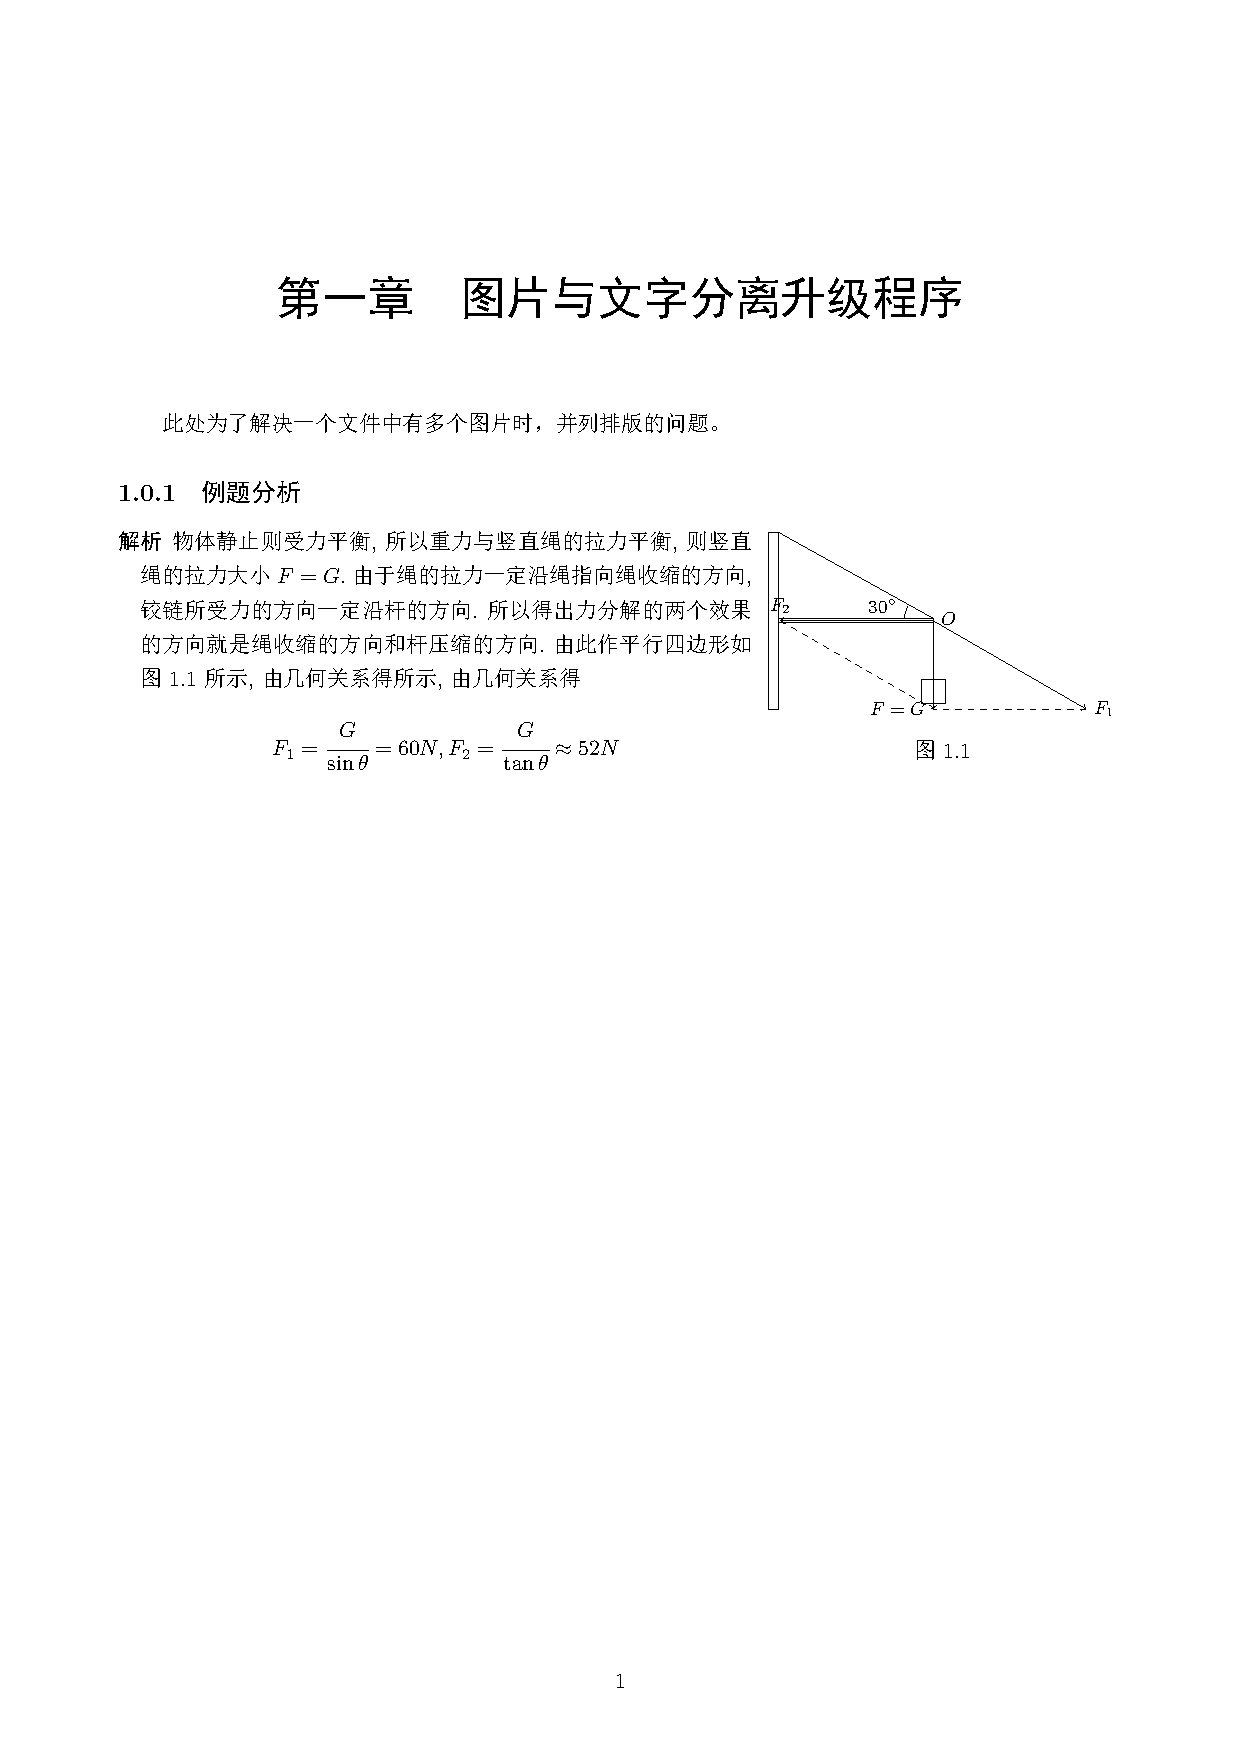
\includegraphics{picture}所示.
%    从下面四个选项中选出正确的选项
%   A.选项A的内容
%   B.选项B的内容
%   C.选项C的内容
%   D.选项D的内容
% 
%  a.AB
% 
%  e.关于选择题正确答案AB的解析.
% 
%  ee.如果解析中有多幅图片,则需要按图片分开来写解析,这一部分是补充,所以没有解析标志.
% 
% \end{choices}
% \end{verbatim}
% 
% 
% \subsection{填空题环境blanks 和 tiankong}
% 
% \begin{function}[added=2019-09-22]{blanks,tiankong}
% blanks 环境(和tiankong 环境相同,只是名称不同而己).如果不加选项[exp],则题目以正常格式排版,如果加上这个选项则以例题来排版,答案不输出到学生模式.在编写程序中考虑到了这一点,这个选项可以是任何作者认为可行的符号,只要给出了选项,则以例题排版.在填空题中以\cs{blank}\Arg{答案} 来标出答案,程序会自动转换成可换行的下划线,同时自动生成答案.在答案输入时以星号*代答案就可以获得正确的答案.
% \end{function}
% 
% \begin{verbatim} 
% \begin{blanks}[exp]
%  1.填空题题干,如果插入图片,则图片应当如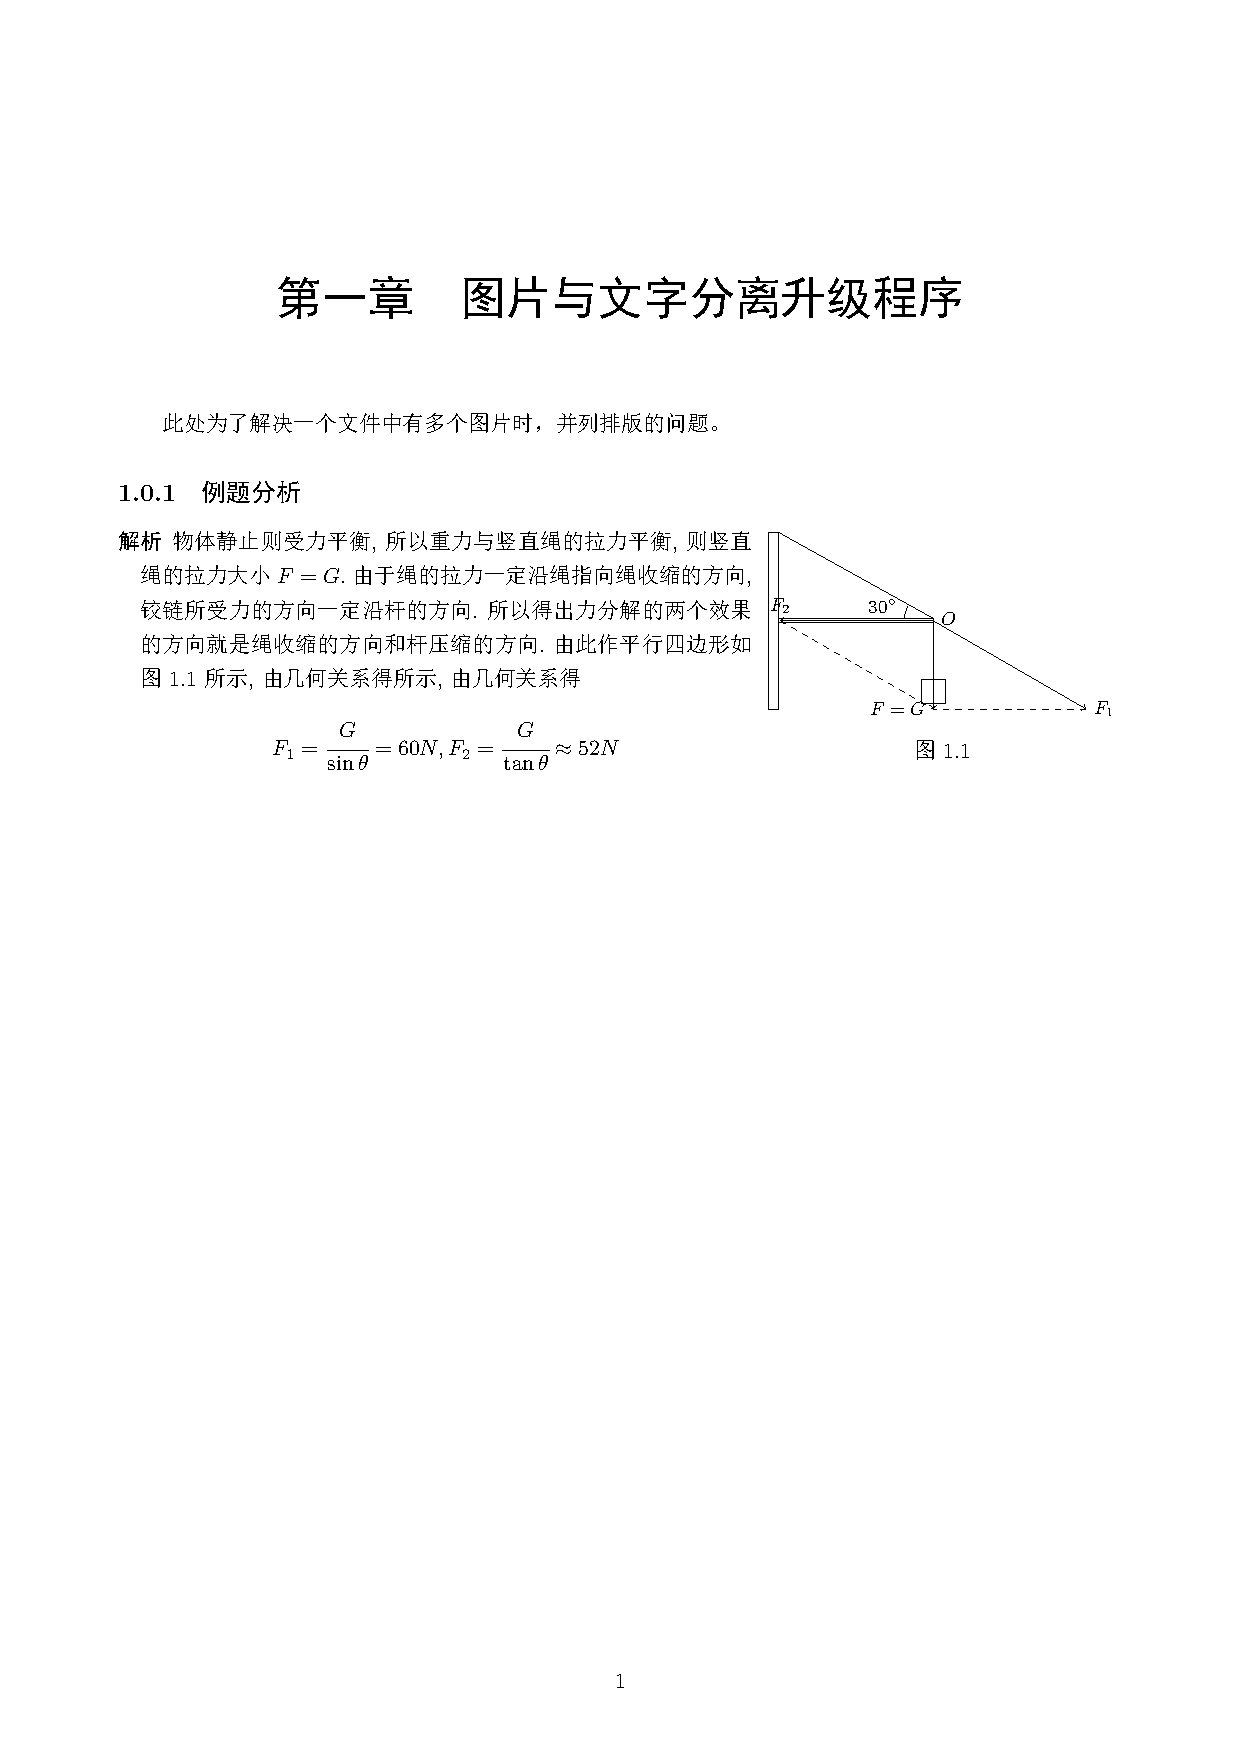
\includegraphics{picture}所示.\blank{答案一}和
%    \blank{答案二}是填空题中需要留出的空白.
% 
%  a.*
% 
%  e.关于填空题正确答案的解析.
% 
%  ee.如果解析中有多幅图片,则需要按图片分开来写解析,这一部分是补充,所以没有解析标志.
% 
% \end{blanks}
% \end{verbatim}
% 
% \subsection{判断题环境judgements 和 panduan}
% 
% \begin{function}[added=2019-09-22]{judgements,panduan}
% judgements 环境(和panduan 环境相同,只是名称不同而己).如果不加选项[exp],则题目以正常格式排版,如果加上这个选项则以例题来排版,答案不输出到学生模式.在编写程序中考虑到了这一点,这个选项可以是任何作者认为可行的符号,只要给出了选项,则以例题排版.答案应当以对应的文字给出,比如:对,错等.
% \end{function}
% 
% \begin{verbatim} 
% \begin{judgements}[exp]
%  1.判断题题干,如果插入图片,则图片应当如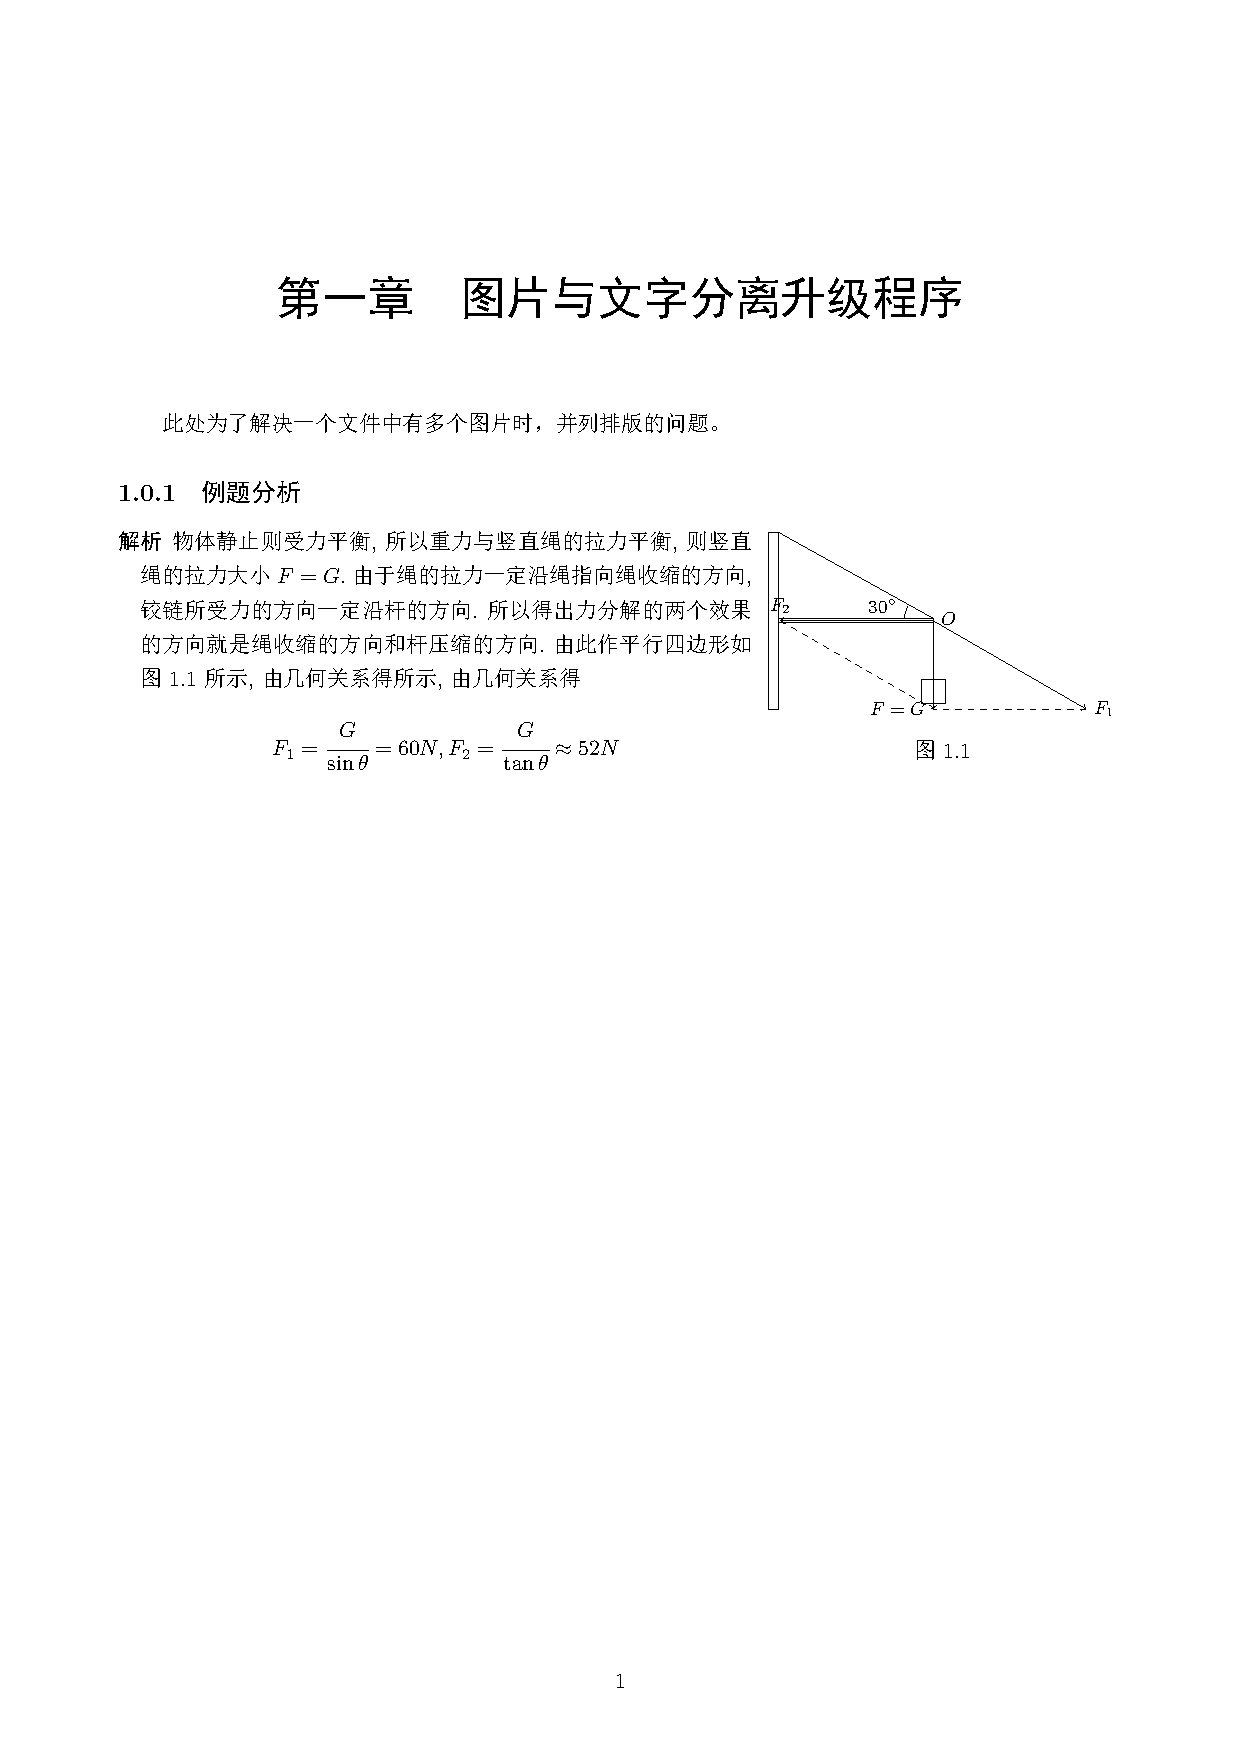
\includegraphics{picture}所示.此问题是正确还是错误
% 
%  a.正确
% 
%  e.关于判断题正确答案的解析.
% 
%  ee.如果解析中有多幅图片,则需要按图片分开来写解析,这一部分是补充,所以没有解析标志.
% 
% \end{judgements}
% \end{verbatim}
% 
% \subsection{计算题环境calculations 和 jisuan}
% 
% \begin{function}[added=2019-09-22]{calculations,jisuan}
% calculations 环境(和jisuan 环境相同,只是名称不同而己).如果不加选项[exp],则题目以正常格式排版,如果加上这个选项则以例题来排版,答案不输出到学生模式.在编写程序中考虑到了这一点,这个选项可以是任何作者认为可行的符号,只要给出了选项,则以例题排版.答案应当以对应的文字给出即可.考虑到有的问题有多个小问,则类比列表环境命令\cs{item}定义了计算题的各小问命令\cs{qitem},这一命令中的$q$ 指的是 \pkg{question}.
% \end{function}
% 
% \begin{verbatim} 
% \begin{calculations}[exp]
%  1.计算题题干,如果插入图片,则图片应当如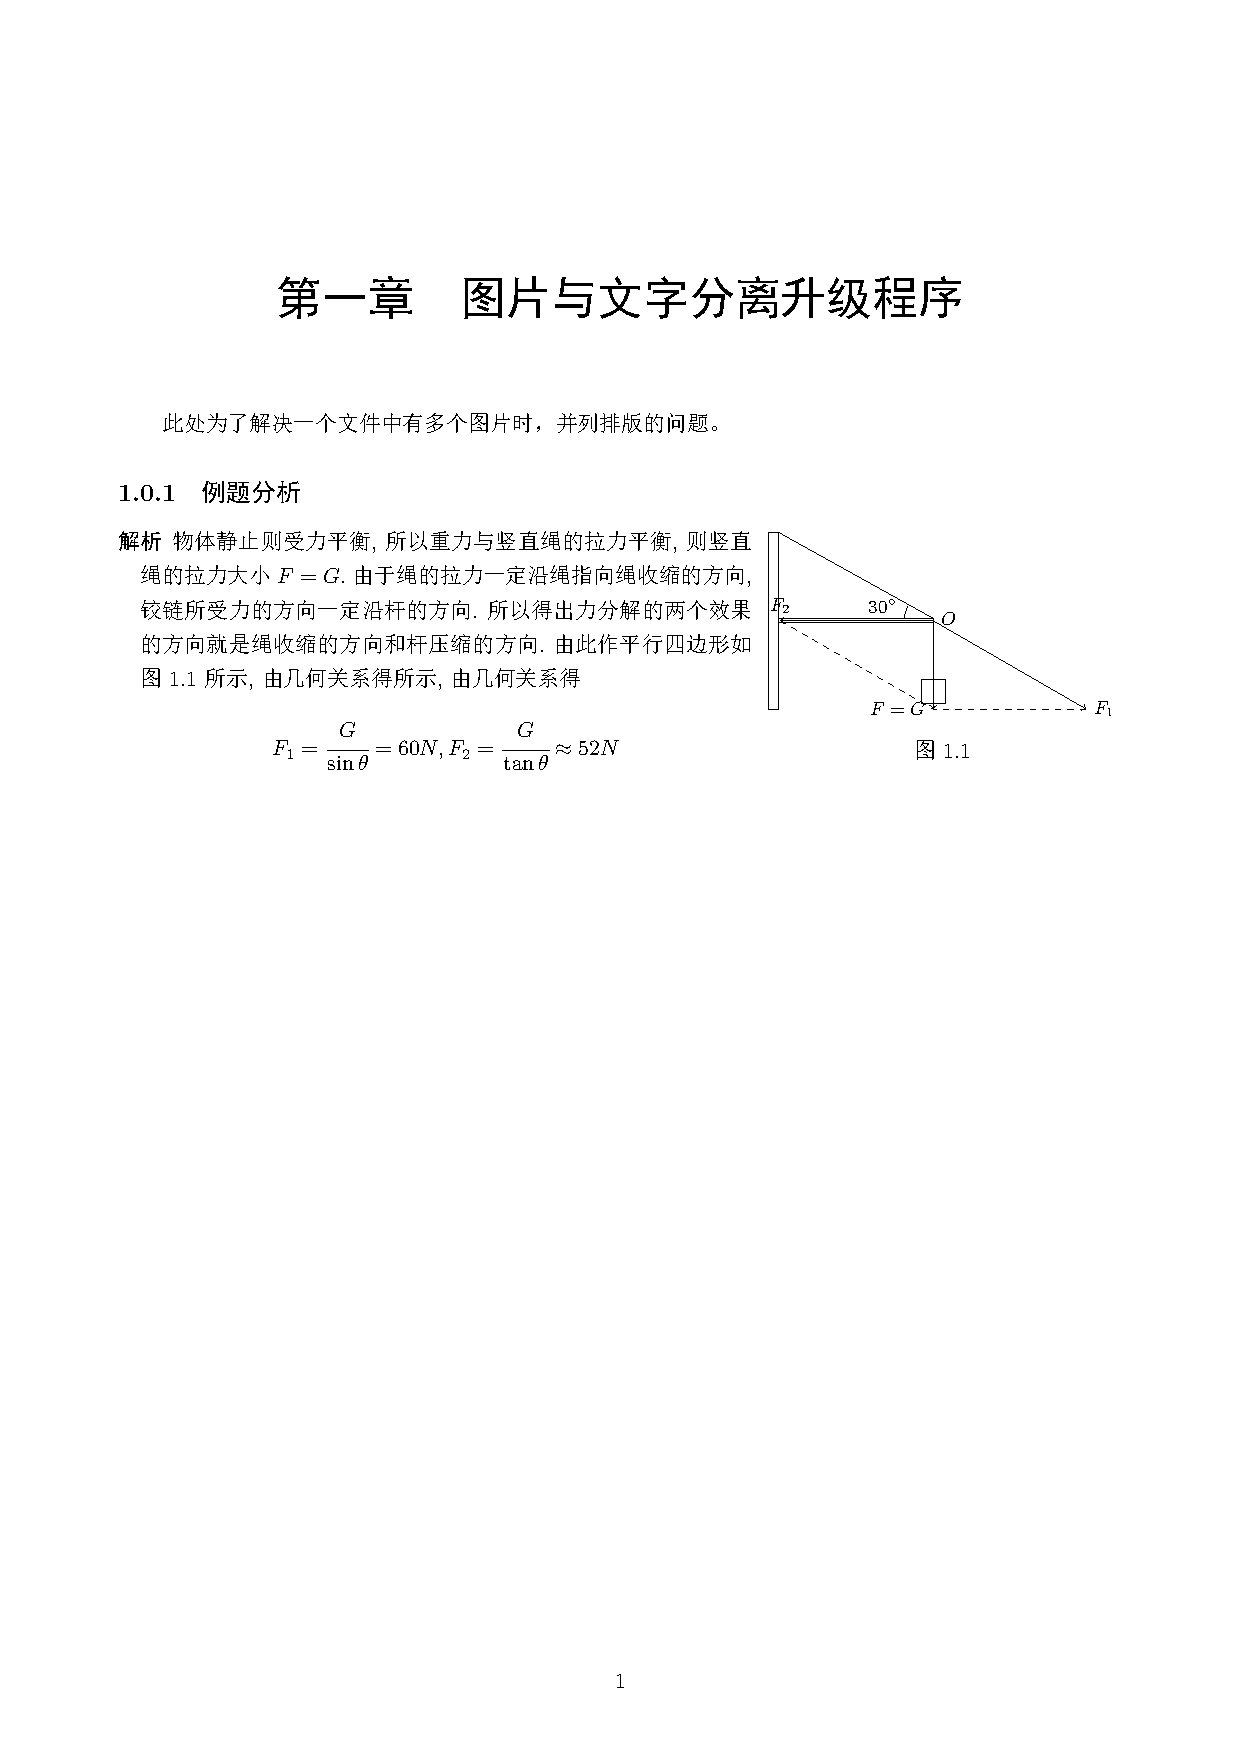
\includegraphics{picture}所示.请求解以下各问题
%  \qitem 第一问的内容
%  \qitem 第二问的内容
%  \qitem ...
% 
%  a.计算题的答案
% 
%  e.关于计算题正确答案的解析.
% 
%  ee.如果解析中有多幅图片,则需要按图片分开来写解析,这一部分是补充,所以没有解析标志.
% 
% \end{calculations}
% \end{verbatim}
% 
% \subsection{首字母下沉命令\cs{lettersink}}
% 
% \begin{function}[added=2019-09-22]{\lettersink}
%  这是一条附加命令,在写完程序后我发现实现这个效果不难,同时该命令支持数学公式的输出,可以实现含数学文本的首字母下沉.
% \end{function}
% 
% \begin{verbatim}
%  \lettersink[首字母高度][首字母与文本间距][首字母颜色]{首字母}
%  其余部分文字,注意这部分文字应当有足够的高度以实现与首字母的绕排.
%  同时默认的首字母高度为2cm,默认与文本间距5pt,默认首字母颜色黑色.
% 
% \end{verbatim}
% 
% \section{各题型排版效果展示}
% 
% \subsection{选择题展示}
%  
% \begin{choices}[exp]
% 1.刻舟求剑的故事家喻户晓,“舟己行矣,而剑不行”这句话所选用的参考系是
% A.舟
% B.地面
% C.舟上的人
% D.流动的水
% 
% a.B
% 
% e.此题考查参考系这一基本概念.舟相对于地行,而剑相对于地静止,所以这句话所选参考系应当为地面.
% 
% 2.某学校田径运动场 $400m$标准跑道如
% \begin{tikzpicture}
%  \draw (-1,0.6)--(1,0.6);
%  \draw (-1,-0.6)--(1,-0.6);
%  \draw (1,-0.6) arc (-90:90:0.6);
%  \draw (-1,0.6) arc (90:270:0.6);
%  \filldraw (-1,0.6) circle [radius=1pt] node [anchor=north] {\small B};
%  \filldraw (1,0.6) circle [radius=1pt]  node [anchor=north] {\small A};
% \end{tikzpicture}
% 所示,$100m$ 赛跑的起跑点在$A$点,终点在$B$点,$400m$ 赛跑的起跑点和终点都在$B$ 点.在校运动会中,甲、乙两位同学分别参加了$100m$ 、$400m$ 项目的比赛,关于甲、
% 乙两位同学运动的位移大小和路程的说法中正确的是
% A.甲、乙的位移大小相等
% B.甲、乙的路程相等
% C.甲的位移比乙大
% D.甲的路比乙大
% 
% a.C
% 
% e.位移是指从初位置到末位置的有向线段,其大小就是有向线段的大小.而路指物体移动轨迹的长度,它是一个标量,所以此题不难考虑出来答案为C.
% 
% 
%  3.下列关于质点的说法中,正确的是
%  A.质点是一个理想化的模型,实际上并不存在,所以引入这个概念没有多大意义
%  B.体积很小的物体更容易看做质点
%  C.凡轻小的物体,皆可看做质点
%  D.当物体的形状和大小对所研究的问题属于无关或者次要因素时,即可把物体看成质点
% 
%  a.D
% 
%  e.建立理想模型是物理中的重要的研究方法,对于复杂问题的研究有重大意义,A错误;一个物体能否看做质点不应看其大小,关键是看其大小对于研究的问题的影响能否忽略,体积很小的物体有时可以看成质点,有时不能看成质点,B错误;一个物体能否看成质点不以轻重而论,C错误;物体能否看成质点取决于其大小和形状对所研究的问题是否属于无关或次要因素,若是就可以看成质点,D正确.
%
% \end{choices}
% 
% 
% \subsection{填空题展示}
% 
% \begin{blanks}[exp]
%  1.打点计时器是记录做直线运动物体的\blank{位移}和\blank{时间}的仪器,电火花计时器是其中的一种,其工作电压是\blank{220v},电火花计时器靠电火花和墨粉打点,当交流电的频率为$50Hz$ 时,它每隔\blank{0.02}秒打一次点。
% 
% a.*
% 
% e.此题考察打点计时器的应用与操作,打点计时器采用打点的方式在纸带上留下点迹,通过测量点迹间的距离可以确定位移。同时使用的电流一定是交流电,它每隔一段时间打一次点,通常频率为$50Hz$ 的交流电,每秒打点50次,所以每两次的间隔为$0.02s$.
% 
% \end{blanks}
% 
% \begin{blanks}
%  1.用 $v-t$ 图像表示小车的运动情况时,以速度$v$ 为\blank{纵轴}、时间 $t$ 为\blank{横轴} 建立直角坐标系,用描点法画出小车的 $v-t$ 图象,图线的 \blank{斜率} 表示加速度的大小,如果 $v-t$ 图象是一条倾斜的直线,说明小车的速度是\blank{均匀变化}的。
% 
% a.*
% 
% e.此题考察 $v-t$ 图象的意义,通过 $v-t$ 图象识别加速度和判断物体运动特征。
% 
% \end{blanks}
% 
% \subsection{判断题展示}
% 
% \begin{judgements}[exp]
%  1.建立直线坐标系时,一定要规定运动方向为正方向
% 
%  a.错误 
% 
%  e.坐标系的建立具有任意性,可以选择任何一 个方向为正方向。但是通常在解决一个实际问题时会根据方便而选择坐标系的方向。
% 
% \end{judgements}
%
% \begin{judgements}
%  2.时间变化量一定为正值
% 
%  a.正确
% 
%  e.变化量指的是末时刻的物理量减去初时刻的物理量,所以时间的变化量一定为正的。
% 
%  3.物体的平均速度为零,则物体一定处于静止状态
% 
%  a.错误 
% 
%  e.当物体转一圈又回到原点时,物体的平均速度为零,但是它却不处于静止状态。
% 
% \end{judgements}
% 
% \subsection{计算题展示}
% 
% \begin{calculations}[exp]
% 
%  2.一物体做匀加速直线运动,通过一段位移$\Delta x$ 所用的时间为$t_1$ ,紧接着通过下一段位移$\Delta x$ 所用时间为$t_2$ ,求物体运动的加速度.
%
%  a.$\cfrac{2\Delta x(t_1-t_2)}{t_1t_2(t_1+t_2)}$
%
%  e.物体通过第一段位移中间时刻的瞬时速度为$v_1=\frac{\Delta x}{t_1}$ ,通过第二段位移中间时刻的瞬时速度为$v_2=\frac{\Delta x}{t_2}$ ,由$v_1$ 变到$v_2$ 所需的时间显然为 $\Delta t=\frac{t_1+t_2}{2}$ ,由加速度定义得
%  $$a=\cfrac{v_2-v_1}{\Delta t}=\cfrac{2\Delta x(t_1-t_2)}{t_1t_2(t_1+t_2)}$$
% 
% 
% \end{calculations}
% 
% \begin{calculations}
% 
%  2.一物体做匀加速直线运动,通过一段位移$\Delta x$ 所用的时间为$t_1$ ,紧接着通过下一段位移$\Delta x$ 所用时间为$t_2$ ,求物体运动的加速度.
%
%  a.$\cfrac{2\Delta x(t_1-t_2)}{t_1t_2(t_1+t_2)}$
%
%  e.物体通过第一段位移中间时刻的瞬时速度为$v_1=\frac{\Delta x}{t_1}$ ,通过第二段位移中间时刻的瞬时速度为$v_2=\frac{\Delta x}{t_2}$ ,由$v_1$ 变到$v_2$ 所需的时间显然为 $\Delta t=\frac{t_1+t_2}{2}$ ,由加速度定义得
%  $$a=\cfrac{v_2-v_1}{\Delta t}=\cfrac{2\Delta x(t_1-t_2)}{t_1t_2(t_1+t_2)}$$
% 
% 
% \end{calculations}
% 
% \subsection{首字母下沉展示}
% 
% \lettersink[2cm][2pt][magenta]
% 物理学的发展,推动了工业、农业和信息技术等方面的进步,引发了一次次的产业革命,改变了人类的生产和生活方式。技术的进步又为物理学的研究提供了更为强大的手段,并引发了人们对物理问题进行更深入的思考,从而反过来促进物理学的发展。
% 创立于17世纪的牛顿力学,被广泛地应用于工程技术,大大推动了社会的发展。18 ~ 19世纪,工程上对蒸汽机的改进需求,又迫使人们对热的问题进行深入研究,引发了热力学的巨大进步。
%  19 ~20世纪初,电磁学的发展,直接导致发电机和无线电通信的诞生,使电能被广泛利用。电走进了千家万户,世界被电灯点亮,电话和电报把各地的人们连接起来,人类从此进入了电气时代。
%
% \section{纯文本和数学文本分离}
% 
% 
% \begin{function}[added=2019-09-19]{\cexam_sep:n}
% 使用此程序来分离纯文本和数学文本,它可以自动探测输入数学文本的模式,支持标准的数学输入格式.分离后将获得三部分:\cs{sep_hd_tl} , \cs{sep_bd_tl}和\cs{sep_tl_tl}.其分别对应头部,数学部和尾部(用来继续生成新的头部和尾部).
% \begin{syntax}
% \cs{cexam_sep:n} \meta{text} \cs{scan_stop:}
% \end{syntax}
% \end{function}
% 
% 
% \section{获得指定宽度文本行数和高度}
% 
% \begin{function}[added=2019-09-19]{\get_par_row:nnn}
% 此程序用来获得文本行数,文本行数存储在所用的\Arg{hang}计数器中.
% 
% \begin{syntax}
% \cs{get_par_row:nnn} \Arg{hang}\Arg{text~width}\Arg{text}
% \end{syntax}
% \end{function}
% 
% \begin{function}[added=2019-09-19]{\get_par_ht:nnn}
% 此程序用来获得文本行数,文本高度存储在所用的\Arg{dim}长度中.
% 
% \begin{syntax}
% \cs{get_par_ht:nnn} \Arg{dim}\Arg{text~width}\Arg{text}
% \end{syntax}
% \end{function}
%
% 
% \begin{function}[added=2019-09-19]{\get_par_rowht:nnnn}
% 此程序用来获得文本行数,文本行数存储在所用的\Arg{hang}计数器中,文本高度存储在所用的\Arg{dim}长度中.
% 
% \begin{syntax}
% \cs{get_par_rowht:nnnn} \Arg{hang}\Arg{dim}\Arg{text~width}\Arg{text}
% \end{syntax}
% \end{function}
% 
% \section{段落形状生成}
% 
% 
% \begin{function}[added=2019-09-20]{\cexam_sha_add:n}
% 用来追加到段落形状中的缩进或者行宽.
% \begin{syntax}
% \cs{cexam_sha_add:n}\Arg{dim}
% \end{syntax}
% \end{function}
% 
% \begin{function}[added=2019-09-20]{\cexam_sha_mk:nnn}
% 此程序用来生成指定缩进和行宽的形状.
% \begin{syntax}
% \cs{cexam_sha_mk:nnn}\Arg{int}\Arg{leftindent}\Arg{linewidth}
% \end{syntax}
% \end{function}
%
% 
% \begin{function}[added=2019-09-20]{\cexam_shad_set:n}
% 设定段落的总行数
% \begin{syntax}
% \cs{cexam_shad_set:n}\Arg{int}
% \end{syntax}
% \end{function}
% 
% 
% \begin{function}[added=2019-09-20]{\cexam_lwr_set:nnnn}
% 设置图片位置及左右缩进.
% 
% \begin{syntax}
% \cs{cexam_lwr_set:nnnn}\Arg{l~or~r}\Arg{picwd}\Arg{lindent}\Arg{rindent}
% \end{syntax}
% \end{function}
% 
% \section{图片格式化}
% 
% 
% \begin{function}[added=2019-09-20]{\cexam_fmt_pic:nnnn}
% 格式化图片命令.
% \begin{syntax}
% \cs{cexam_fmt_pic:nnnn}\Arg{l~or~r}\Arg{pic}\Arg{lindent}\Arg{rindent}
% \end{syntax}
% \end{function}
% 
% \section{基本排版程序}
% 
% 
% \begin{function}[added=2019-09-20]{\cexam_type_i:nnnnnnn}
% 此程序用以排版文本以行宽减图宽排版时高度大于图高的情况,其第一级和第二级缩进可以单独设置,由于没有第三级缩进所以此不能用于排版选择题含长选项的情况,因为长选项是第三级部分,其是需要缩进的.但是当选项不是长选项时,其不需要缩进,则要以此程序排版.
% \begin{syntax}
% \cs{cexam_type_i:nnnnnnn}
% \Arg{l~or~r}\Arg{pic}
% \Arg{lind}\Arg{rind}
% \Arg{sublind}\Arg{subrind}
% \Arg{text}
% \end{syntax}
% \end{function}
% 
% 
% \begin{function}[added=2019-09-21]{\cexam_type_ii:nnnnnnnnn}
% 此程序用以排版文本以行宽减图宽排版时高度大于图高的情况,其第一级,第二级和第三级缩进可以单独设置,于排版选择题含长选项的情况,因为长选项是第三级部分,其是需要缩进的.其也可以排版选择题短选项,即第三级缩进同第二级缩进相同的情况,但是这样会执行更多的代码,对于短选项部分使用\cs{cexam_type_i:nnnnnnn} 排版更加合理.
% \begin{syntax}
% \cs{cexam_type_ii:nnnnnnnnn}
%  \Arg{l~or~r}\Arg{pic}
%  \Arg{lind}\Arg{rind}
%  \Arg{sublind}\Arg{subrind}
%  \Arg{subsublind}\Arg{subsubrind}
%  \Arg{text}
% \end{syntax}
% \end{function}
% 
% 
% \begin{function}[added=2019-09-21]{\cexam_type_iii:nnnnnnn}
% 此程序用以排版题干,图片居中,选项依次排版的情况.
% \begin{syntax}
% \cs{cexam_type_iii:nnnnnnn}
%  \Arg{l~or~r}\Arg{pic}
%  \Arg{lind}\Arg{rind}
%  \Arg{sublind}\Arg{subrind}
%  \Arg{text}
% \end{syntax}
% \end{function}
% 
% 
% \begin{function}[added=2019-09-21]{\cexam_type_iv:nnnnnnnn}
% 此程序用以排版含图模式,其含有二部分文本,第一部分为题干第二部分为选项(选择题长选项)且这二级缩进可以单独设置.
% \begin{syntax}
% \cs{cexam_type_iv:nnnnnnnn}
%  \Arg{l~or~r}\Arg{pic}
%  \Arg{lind}\Arg{rind}
%  \Arg{sublind}\Arg{subrind}
%  \Arg{text}\Arg{subtext}
% \end{syntax}
% \end{function}
% 
% 
% \begin{function}[added=2019-09-21]{\cexam_type_v:nnnnn}
% 此程序用以排版无图模式,包含二级缩进,这二级的左右缩进可以单独设置.
% \begin{syntax}
% \cs{cexam_type_v:nnnnn}
%  \Arg{lind}\Arg{rind}
%  \Arg{sublind}\Arg{subrind}
%  \Arg{text}
% \end{syntax}
% \end{function}
% 
% \StopEventually{}
% 
%\begin{implementation}
% \clearpage
% \section{代码实现}
%
% \subsection{缩写列表}
% 
% 由于编写过程中需要对函数命名,如果为了清析则可以使用全称来命名,但是这样做会导致程序的名字过长,输入不便同时会影响逻辑结构的表达清析.但是用过短的简写来命名,对于维护来说不是很方便,这也是我在此处列出缩写列表的目的所在,两者兼顾,同时所生成的宏包还不容易被破译.
%
%  \begin{center}
%  \begin{tabular}{|*{12}{c|}}
%  \hline
%  简写&英文&中文&&简写&英文&中文&&简写&英文&中文\\
%  \hline
%  by& body&主体&& mk& make& 生成&& rec&rectangle&矩形\\
%  \hline
%  hd&head&头部&& sha&shape&形状&&sep&separate&分离\\
%  \hline
%  tl&tail&尾部&&txt &text &文本 &&mat &math &数学 \\
%  \hline
%  sub&subtraction&减去&&ps &parshape&形状&&equ &equation &公式 \\
%  \hline
%  \end{tabular}
%  \end{center}
%
% \subsection{布尔值设置}
%    \begin{macrocode}
%<*package>
%    \end{macrocode}
%
%    \begin{macrocode}
%<@@=cexam>
%    \end{macrocode}
%  \pkg{expl3}和\pkg{l3keys2e}检测,设置此检测的目的是:随着\pkg{cexam}的开发,将来有可能用到这两个宏包的新增功能,而旧版有可能不包含新的功能,所以要检测一下版本日期,确保存在需要的新功能,为了不依赖于\pkg{ctex}这里直接借用其检测代码。
%
% \begin{macro}[added=2020/05/01]{l3-too-old}
% \changes{v3.2.6}{2020/05/01}{新增版本检测}
%    \begin{macrocode}
\msg_new:nnnn {cexam}{l3-too-old}
{Support~package~#1~too~old.}
{
   Please~update~an~up~to~date~version~of~the~bundles\\\\
   'l3kernel'~and~'l3packages'\\\\
   using~your~TeX~package~manager~or~from~CTAN
}
\@ifpackagelater{expl3}{2019/03/05}{}
{\msg_error:nnn {cexam}{l3-too-old}{expl3}}
\@ifpackagelater{l3keys2e}{2015/12/20}{}
{\msg_error:nnn {cexam}{l3-too-old}{l3keys2e}}
%    \end{macrocode}
% \end{macro}
% 
%    \begin{variable}[added=2019-05-11]{\g_@@_sep_bd_bool,\g_@@_sep_tl_bool}
%  这两个布尔值在数学分离模式中标志数学模式是否文本串中有数学公式,字符串分离后尾部是否为空.
%    \begin{macrocode}
\bool_new:N \g_@@_sep_bd_bool
\bool_new:N \g_@@_sep_tl_bool
%    \end{macrocode}
%    \end{variable}
%
%    \begin{variable}[added=2019-08-25]{\cexam_nopic_bool,\cexam_notab_bool}
%  此二个布尔值用来判断图片与文字分离时,题干中是否存在图片(或表格).如果为真则无图片(或表格),如果为假,则有图片.
%    \begin{macrocode}
\bool_new:N \cexam_nopic_bool
\bool_new:N \cexam_notab_bool
%    \end{macrocode}
%    \end{variable}
%
%    \begin{variable}[added=2019-08-29]{\cexam_fmt_bool}
% \changes{v3.1.2}{2019/08/29}{增加图片格式化判断布尔值}
%  此布尔值用来判断图片是否需要格式化,即带上下标号.
%
%    \begin{macrocode}
\bool_new:N \cexam_fmt_bool
%    \end{macrocode}
%    \end{variable}
%
%    \begin{variable}[added=2019-08-29]{\cho_opt_maxed_bool}
% \changes{v3.1.2}{2019/08/29}{增加长选项判断布尔值}
%  此布尔值用来判断选择题选项是否是按长行依次排列.
%
%    \begin{macrocode}
\bool_new:N \cho_opt_maxed_bool 
%    \end{macrocode}
%    \end{variable}
%
%    \begin{variable}[added=2019-08-29]{\cho_data_bool}
% \changes{v3.1.2}{2019/08/29}{增加长选项判断布尔值}
%  此布尔值用来判断选择题的结构是否完整.
%
%    \begin{macrocode}
\bool_new:N \cho_data_bool
%    \end{macrocode}
%    \end{variable}
%
%    \begin{variable}[added=2019-09-18]{\answer_student_bool}
% \changes{v3.1.6}{2019/09/18}{增加学生模式答案写出布尔值}
%  此布尔值用来判断是否是学生模式,当为学生模式时答案不在原题显示,而在书籍后面生成单独的答案.
%
%    \begin{macrocode}
\bool_new:N \answer_student_bool
%    \end{macrocode}
%    \end{variable}
%
% \subsection{盒子设置}
%
% \begin{variable}[added=2019-05-14]{\cexam_txtht_box}
% 此盒子用来在计算行数时获得对应文字的高度,其应用于测量高度时接收\cs{parbox}的预排版. 
%    \begin{macrocode}
\box_new:N \cexam_txtht_box
%    \end{macrocode}
% \end{variable}
%
% \begin{variable}[added=2019-08-14]{\cexam_picture_box}
% 此盒子用来存储图片,以获得图片的各种尺寸.
%    \begin{macrocode}
\box_new:N \cexam_picture_box 
%    \end{macrocode}
% \end{variable}
%
% \begin{variable}[added=2019-08-24]{\cho_option_box}
% \changes{v3.0.9}{2019/08/24}{新增选择题选项最大长度获取盒子}
% 此盒子用来存储选择题中的选项,以获得选项单行排版时的宽度.
%    \begin{macrocode}
\box_new:N \cho_option_box
%    \end{macrocode}
% \end{variable}
%
% \begin{variable}[added=2019-08-25]{\cexam_option_box}
% \changes{v3.1.0}{2019/08/25}{新增选项格式化盒子}
% 此盒子用来存储格式化的选项,用来的最终排版时生成对应的段落格式.
%    \begin{macrocode}
\box_new:N \cexam_option_box
%    \end{macrocode}
% \end{variable}
%
% \begin{variable}[added=2019-08-25]{\sep_temp_box}
% \changes{v3.1.0}{2019/08/25}{新增图片分离临时盒子}
% 此盒子用来在分离图片和文本时临时存储图片,以判定图片是否为空.
%    \begin{macrocode}
\box_new:N \sep_temp_box
%    \end{macrocode}
% \end{variable}
%
% \begin{variable}[added=2019-08-29]{\cho_optpic_box}
% \changes{v3.1.2}{2019/08/29}{新增判定选项排版格式盒子}
%
% 此盒子用来存储决定选项排版时,图片的各尺寸,为了防止与图片格式化时的付值影响图片格式化,所以此处单独设置一个盒子.
%    \begin{macrocode}
\box_new:N \cho_optpic_box
%    \end{macrocode}
% \end{variable}
%
% \begin{variable}[added=2019-08-29]{\cexam_number_box}
% \changes{v3.1.2}{2019/08/29}{新增题号格式尺寸获得盒子}
%
%    \begin{macrocode}
\box_new:N \cexam_number_box
%    \end{macrocode}
% \end{variable}
%
% \begin{variable}[added=2019-09-03]{\blank_wd_box}
% \changes{v3.1.3}{2019/09/03}{新增填空题空白长度测量盒子}
%
%    \begin{macrocode}
\box_new:N \blank_wd_box
%    \end{macrocode}
% \end{variable}
%
% \begin{variable}[added=2020-03-22]{\fmt_picture_box,\fmt_picture_vbox,\fmt_picture_hbox,\fmt_pic_vbox,\fmt_pic_hbox,\fmt_pic_r_hbox,\fmt_pic_r_vbox,\fmt_pic_t_vbox}
% \changes{v3.2.4}{2020/03/22}{新增前缀盒子}
%  
% 此盒子是在前缀设置命令\cs{cexam_fmt_pic:nnnn}中为了取代之前的\cs{parbox}命令而专门设置了,它们用来构建图片的放置位置。
%
%    \begin{macrocode}
\box_new:N \fmt_picture_box
\box_new:N \fmt_picture_vbox
\box_new:N \fmt_picture_hbox
\box_new:N \fmt_pic_vbox
\box_new:N \fmt_pic_hbox
\box_new:N \fmt_pic_r_hbox
\box_new:N \fmt_pic_r_vbox
\box_new:N \fmt_pic_t_vbox
%    \end{macrocode}
% \end{variable}
%
% \begin{variable}[added=2020-03-27]{\ind_hat_vbox ,\ind_hat_hbox ,\ind_hat_box}
% \changes{v3.2.5}{2020/03/27}{新增前缀盒子}
%  
% 此盒子是在前缀设置命令\cs{cexam_ind_hat:nnnn}中为了取代之前的\cs{parbox}命令而专门设置了,它们用来构建前缀。
%    \begin{macrocode}
\box_new:N \ind_hat_vbox
\box_new:N \ind_hat_hbox
\box_new:N \ind_hat_box
%    \end{macrocode}
% \end{variable}
%
% \subsection{长度设置}
%
% \begin{variable}[added=2019-07-31]{\rec_tempht_dim}
% 此长度变量用来在计算行数时,临时存储文本的高度.
%    \begin{macrocode}
\dim_new:N \rec_tempht_dim
%    \end{macrocode}
% \end{variable}
%
% \begin{variable}[added=2019-07-31]{\cexam_psrin_dim,\cexam_pslin_dim,\cexam_pswd_dim}
% 此三个变量用来在形状生成程序中存储右缩进,左缩进,行宽.
%    \begin{macrocode}
\dim_new:N \cexam_psrin_dim 
\dim_new:N \cexam_pslin_dim 
\dim_new:N \cexam_pswd_dim 
%    \end{macrocode}
% \end{variable}
%
% \begin{variable}[added=2019-08-14]{\cexam_picht_dim,\cexam_picwd_dim}
% 此三个变量用来处理图片时记录图片的高,宽.第三个长是为了进行三级排版时设置的.
%    \begin{macrocode}
\dim_new:N \cexam_picht_dim
\dim_new:N \cexam_picwd_dim
%    \end{macrocode}
% \end{variable}
%
% \begin{variable}[added=2019-08-24]{\cho_lmax_dim}
% \changes{v3.0.9}{2019/08/24}{选择题最大选项长度}
% 此长度用来存储选择题中四个选项的最大长度
%    \begin{macrocode}
\dim_new:N \cho_lmax_dim
\dim_set:Nn \cho_lmax_dim {0pt}
%    \end{macrocode}
% \end{variable}
%
% \begin{variable}[added=2019-10-10]{\cho_lmax_i_dim ,\cho_lmax_ii_dim}
% \changes{v3.1.9}{2019/10/10}{新增\cs{cho_lmax_i_dim}}
% \changes{v3.2.0}{2019/10/13}{新增\cs{cho_lmax_ii_dim}}
% \cs{cho_lmax_i_dim}来存储选择题中A选项和B选项中的最大宽度,
% \cs{cho_lmax_ii_dim}来存储选择题中C选项和D选项中的最大宽度
%
%    \begin{macrocode}
\dim_new:N \cho_lmax_i_dim
\dim_new:N \cho_lmax_ii_dim
\dim_set:Nn \cho_lmax_i_dim {0pt}
\dim_set:Nn \cho_lmax_ii_dim {0pt}
%    \end{macrocode}
% \end{variable}
%
% \begin{variable}[added=2019-08-25]{\cho_optwd_dim,\cho_optwd_i_dim}
% \changes{v3.1.0}{2019/08/25}{选择题选项的行宽}
% 第一个长度用来存储选择题四个选项排版时的行宽,默认值为\cs{linewidth}
% 第二个长度用来确定每个选项的排版宽度
%
%    \begin{macrocode}
\dim_new:N \cho_optwd_dim
\dim_new:N \cho_optwd_i_dim
%    \end{macrocode}
% \end{variable}
%
% \begin{variable}[added=2019-08-29]{\sep_HD_ht}
% \changes{v3.1.2}{2019/08/29}{新增长度}
% 此长度用来存储已经排过版的内容的高度,用以辅助生成文本高度和行数.
%    \begin{macrocode}
\dim_new:N \sep_HD_ht  
%    \end{macrocode}
% \end{variable}
%
% \begin{variable}[added=2019-08-29]{\cho_optpic_wd_dim,\cho_optpic_ht_dim,\cho_optpic_hti_dim}
% \changes{v3.1.2}{2019/08/29}{新增长度}
% 第一个长度用来存储选择题选项的宽度,第二个用来存储选项的高度,第三个用来存储判断高度
%    \begin{macrocode}
\dim_new:N \cho_optpic_ht_dim
\dim_new:N \cho_optpic_hti_dim
\dim_new:N \cho_optpic_wd_dim
%    \end{macrocode}
% \end{variable}
%
% \begin{variable}[added=2019-08-29]{\cexam_indent_dim,\cexam_indent_i_dim}
% \changes{v3.1.2}{2019/08/29}{新增长度}
% 第一个长度用来存储一级缩进,第二个用来存储二级缩进.
%    \begin{macrocode}
\dim_new:N \cexam_indent_dim
\dim_new:N \cexam_indent_i_dim
%    \end{macrocode}
% \end{variable}
%
% \begin{variable}[added=2019-09-01]{\cexam_pictxt_skip,\cexam_numtxt_skip}
% \changes{v3.1.2}{2019/09/01}{新增长度}
% 第一个长度用来存储图片与文本的间距,第二个用来存储题号与文本的间距.默认值都是5pt.
%    \begin{macrocode}
\dim_new:N \cexam_pictxt_skip 
\dim_set:Nn \cexam_pictxt_skip{5pt}
\dim_new:N \cexam_numtxt_skip
\dim_set:Nn \cexam_numtxt_skip{5pt}
%    \end{macrocode}
% \end{variable}
%
% \begin{variable}[added=2019-09-03]{\cexam_pic_linwd_dim}
% \changes{v3.1.3}{2019/09/03}{新增长度}
% 此长度为格式化图片时的行宽.
%
%    \begin{macrocode}
\dim_new:N \cexam_pic_linwd_dim
%    \end{macrocode}
% \end{variable}
%
% \begin{variable}[added=2019-09-03]{\blank_wd_dim}
% \changes{v3.1.3}{2019/09/03}{新增长度}
% 此长度为填空题生成空白的答案的长度.
%
%    \begin{macrocode}
\dim_new:N \blank_wd_dim
%    \end{macrocode}
% \end{variable}
%
% \begin{variable}[added=2019-09-10]{\get_rec_linewd_dim}
% \changes{v3.1.3}{2019/09/10}{新增长度}
% 此长度为生成矩形行数时的专有长度,不与其它程序共用.
%
%    \begin{macrocode}
\dim_new:N \get_rec_linewd_dim
%    \end{macrocode}
% \end{variable}
% 
% \begin{variable}[added=2019-09-27]{\cexam_picwd_limit}
% \changes{v3.1.9}{2019/09/27}{新增长度}
% 此命令用来限制图片宽度,设置为行宽的一半,如果超过一半则使用 \cs{cexam_type_iii:nnnnnnn} 排版.
%
%    \begin{macrocode}
\dim_new:N \cexam_picwd_limit 
%    \end{macrocode}
% \end{variable}
% 
% \begin{variable}[added=2020-05-01]{\cexam_ccwd_dim}
% \changes{v3.2.6}{2020/05/01}{新增长度\cs{cexam_ccwd_dim},取消对\pkg{ctex}的依赖}
%
%    \begin{macrocode}
\dim_new:N \cexam_ccwd_dim
\cs_if_exist:NTF \ccwd 
{\dim_set:Nn \cexam_ccwd_dim {\ccwd}}
{\dim_set:Nn \cexam_ccwd_dim {1em}}
%    \end{macrocode}
% \end{variable}
% 
% \begin{variable}[added=2019-10-20]{\cho_hat_dim , \cho_hat_wd_dim,\cho_hat_ht_dim}
% \changes{v3.2.1}{2019/10/20}{新增长度}
% \changes{v3.2.5}{2020/03/27}{新增长度\cs{cho_hat_ht_dim}}
% 此命令用来设置选择题四个选项与A,B,C,D的间隔。不论何种排版可以达到一致的效果。
%
%    \begin{macrocode}
\dim_new:N \cho_hat_dim
\dim_new:N \cho_hat_wd_dim
\dim_set:Nn \cho_hat_dim {.3\cexam_ccwd_dim}
\dim_set:Nn \cho_hat_wd_dim {1.2\cexam_ccwd_dim}
\dim_add:Nn \cho_hat_wd_dim {\cho_hat_dim}
\dim_new:N \cho_hat_ht_dim 
\dim_set:Nn \cho_hat_ht_dim {.7\cexam_ccwd_dim}
%    \end{macrocode}
% \end{variable}
%
% \begin{variable}[added=2020-02-22]{\fmt_pic_t_xdim,\fmt_pic_t_ydim,\fmt_picture_xdim,\fmt_picture_ydim}
% \changes{v3.2.4}{2020/03/22}{新增长度用来在格式化图片时定位图片位置}
%
%    \begin{macrocode}
\dim_new:N \fmt_pic_t_xdim
\dim_new:N \fmt_pic_t_ydim 
\dim_new:N \fmt_picture_xdim
\dim_new:N \fmt_picture_ydim
%    \end{macrocode}
% \end{variable}
% 
% \subsection{计数器设置}
%
% \begin{variable}[added=2019-08-29]{\cexam_number_int}
% \changes{v3.1.2}{2019/08/29}{新增题号计数器}
%
%    \begin{macrocode}
\int_new:N \cexam_number_int
%    \end{macrocode}
% \end{variable}
%
% \begin{variable}[added=2019-08-03]{\cexam_equ_int}
% 此计数器用来在测行时,数学公式的计数器会增加,所以此计数器对数学公式部分取得高度后数学公式计数器的还原.
%
%    \begin{macrocode}
\int_new:N \cexam_equ_int
%    \end{macrocode}
% \end{variable}
%
% \begin{variable}[added=2019-08-14]{\cexam_numtemp_int}
% 此计数器在计算行数时,临时使用.
%
%    \begin{macrocode}
\int_new:N  \cexam_numtemp_int
%    \end{macrocode}
% \end{variable}
%
% \begin{variable}[added=2019-08-14]{\cexam_picmath_int,\cexam_totalnum_int}
% 此二计数器分别记录图片的高度所生成的行数,图片之后一级,二级缩进的总行数,
%
%    \begin{macrocode}
\int_new:N \cexam_picmath_int
\int_new:N \cexam_totalnum_int
%    \end{macrocode}
% \end{variable}
%
% \begin{variable}[added=2019-09-03]{\cexam_qitem_int}
% \changes{v3.1.3}{2019/09/03}{新增计算题小问计数器}
%
%    \begin{macrocode}
\int_new:N \cexam_qitem_int
%    \end{macrocode}
% \end{variable}
% 
% \begin{variable}[added=2019-09-19]{\example_number_int,\cexam_numold_int}
% \changes{v3.1.7}{2019/09/19}{新增存储题号计数器和例题环境题号计数器}
%
%    \begin{macrocode}
\int_new:N \example_number_int
\int_new:N \cexam_numold_int
%    \end{macrocode}
% \end{variable}
%
% \subsection{字符串变量}
% 
% \begin{macro}[added=2019-02-16]{\sep_hd_tl , \sep_bd_tl ,\sep_tl_tl}
% \changes{v3.2.2}{2019/02/16}{新增字符串变量}
% 
% 此处所设置字符串变量用于数学文本和常规文本的分离中,及生成矩形行数时累加字符串头部内容。
%    \begin{macrocode}
\tl_new:N\sep_hd_tl
\tl_new:N\sep_bd_tl
\tl_new:N\sep_tl_tl
\tl_new:N\sep_HD_tl
%    \end{macrocode}
% \end{macro}
% 
% \begin{macro}[added=2019-02-16]{\cho_fmt_tl}
% \changes{v3.2.2}{2019/02/16}{新增字符串变量}
% 选择题格式化时所加空白
% 
%    \begin{macrocode}
\tl_new:N\cho_fmt_tl
%    \end{macrocode}
% \end{macro}
% 
% 
% \begin{macro}[added=2019-02-16]{\cexam_number_tag_tl ,\cexam_number_tag_i_tl}
% \changes{v3.2.2}{2019/02/16}{新增字符串变量}
% 此处字符串为题目的编号 
%    \begin{macrocode}
\tl_new:N \cexam_number_tag_tl
\tl_new:N \cexam_number_tag_i_tl
%    \end{macrocode}
% \end{macro}
% 
% 
% \begin{macro}[added=2019-02-16]{\ans_tag_tl ,\ana_tag_tl , \ans_tag_i_tl ,\ans_tag_i_tl}
% \changes{v3.2.2}{2019/02/16}{新增字符串变量}
% 此处字符串为答案和解析的格式
% 
%    \begin{macrocode}
\tl_new:N \ans_tag_tl
\tl_new:N \ans_tag_i_tl
\tl_new:N \ana_tag_tl
\tl_new:N \ana_tag_i_tl
%    \end{macrocode}
% \end{macro}
% 
% 
% \begin{macro}[added=2020-07-14]{\prf_tag_tl,\prf_tag_i_tl,\prf_end_tl}
% \changes{v3.2.8}{2020/07/14}{新增证明题标签}
%
%    \begin{macrocode}
\tl_new:N \prf_tag_tl
\tl_new:N \prf_tag_i_tl
\tl_new:N \prf_end_tl
%    \end{macrocode}
% \end{macro}
%
% \begin{macro}[added=2019-02-16]{\cexam_blank_tl ,\cexam_quad_tl}
% \changes{v3.2.2}{2019/02/16}{新增字符串变量}
% 存储填空题答案
%    \begin{macrocode}
\tl_new:N \cexam_blank_tl
\tl_const:Nn\cexam_quad_tl {\rule[-2pt]{\cexam_ccwd_dim}{0.4pt}}
%    \end{macrocode}
% \end{macro}
%
% \begin{macro}[added=2019-08-15]{\cexam_fmt_tag_tl,\cexam_picture_tl}
%
% 此字符串存储了图片编号的格式,如果需要修改,则可以修改这个命令.
%    \begin{macrocode}
\tl_new:N \cexam_fmt_tag_tl
\tl_new:N \cexam_picture_tl
%    \end{macrocode}
% \end{macro}
%
% \begin{macro}[added=2020-03-28]{\cexam_shape_tl}
%
% 此字符串存储了段落的形状,曾经使用\cs{cs_new:Nn}来写的,此处定义更加合理。
%    \begin{macrocode}
\tl_new:N \cexam_shape_tl
%    \end{macrocode}
% \end{macro}
%
% \subsection{宏包选项}
% 
% \begin{macro}[added=2019-09-18]{\answer_write}
% \changes{v3.1.6}{2019/09/18}{新增答案写出}
%
% 答案写出命令
%    \begin{macrocode}
\iow_new:N \answer_write
%    \end{macrocode}
% \end{macro}
% 
% \begin{macro}[added=2019-09-18]{cexam/option}
% \changes{v3.1.6}{2019/09/18}{新增宏包选项}
% 宏包选项,学生模式为答案单独写出,老师模式为不写出答案而在原题显示.
%
%    \begin{macrocode}
\keys_define:nn {cexam / option}
{
   user  .code:n = 
   {
      \str_if_in:nnTF {#1}{student}
      {
	 \bool_set_true:N \answer_student_bool
	 \iow_open:Nn \answer_write {\jobname.ans}
      }
      {\bool_set_false:N \answer_student_bool}
   }
}
\ProcessKeysOptions {cexam / option}
%    \end{macrocode}
% \end{macro}
%
% \subsection{文本和数学分离}
% 
% \begin{macro}[added=2019-05-10]{\cexam_sep_i:n , \cexam_sep_ii:n, \cexam_sep_iii:n}
%
% 三个基本数学模式分离,数学模式符号不处于字符串两端的处理
% \changes{v3.2.2}{2019/02/16}{用\LaTeXiii{}中的数据格式tokenlist 重写了数据分析结构}
%
%    \begin{macrocode}
\cs_new:Npn \cexam_sep_i:n  #1$$#2$$#3\scan_stop:
{
  \tl_set:Nn \sep_hd_tl {#1}
  \tl_set:Nn \sep_bd_tl {$$#2$$}
  \tl_set:Nn \sep_tl_tl {#3}
}
%
\cs_new:Npn \cexam_sep_ii:n #1\[#2\]#3\scan_stop:
{
  \tl_set:Nn \sep_hd_tl {#1}
  \tl_set:Nn \sep_bd_tl {\[#2\]}
  \tl_set:Nn \sep_tl_tl {#3}
}
%
\cs_new:Npn \cexam_sep_iii:n #1\begin#2\end#3#4\scan_stop:
{
  \tl_set:Nn \sep_hd_tl {#1}
  \tl_set:Nn \sep_bd_tl {\begin#2\end{#3}}
  \tl_set:Nn \sep_tl_tl {#4}
}
%    \end{macrocode}
% \end{macro}
%
% \begin{macro}[added=2019-05-10]{\cexam_sep_mk:n}
% 将三个数学模式合并为一个处理程序
%    \begin{macrocode}
\cs_new:Npn \cexam_sep_mk:n #1\scan_stop:
{
  \str_if_in:nnTF {#1}{$$}%$$
  {\cexam_sep_i:n #1\scan_stop:}
  {
    \str_if_in:nnTF {#1}{\[}%\]
      {\cexam_sep_ii:n #1\scan_stop:}
      {
	  \str_if_in:nnTF {#1}{\begin}
	  {\cexam_sep_iii:n #1\scan_stop:}
	  {}
      }
  }
}
%    \end{macrocode}
% \end{macro}
% \begin{macro}[added=2019-05-10]{\cexam_sep_isin:nn}
% 加入三个数学模式符号处于字符串两端的处理
% \changes{v3.2.2}{2019/02/16}{用\LaTeXiii{}中的数据格式tokenlist 重写了数据分析结构}
%    \begin{macrocode}
  \cs_new:Npn \cexam_sep_isin:nn #1#2
  {
    \str_if_in:nnTF {*#1}{*#2}
    {
      \bool_set_true:N \g_@@_sep_bd_bool
      \str_if_in:nnTF {#1*}{#2*}
      {
	 \tl_set:Nn \sep_hd_tl {}
	 \tl_set:Nn \sep_bd_tl {}
	 \tl_set:Nn \sep_tl_tl {}
	 \bool_set_false:N \g_@@_sep_tl_bool
      }
      {
	\cexam_sep_mk:n *#1\scan_stop:
	\tl_set:Nn \sep_hd_tl {}
	\bool_set_true:N \g_@@_sep_tl_bool
      }
    }
    {
      \str_if_in:nnTF {#1*}{#2*}
      {
	\bool_set_true:N \g_@@_sep_bd_bool
	\cexam_sep_mk:n #1*\scan_stop:
	\tl_set:Nn \sep_hd_tl {}
	\bool_set_false:N \g_@@_sep_tl_bool
      }
      {
	\str_if_in:nnTF {#1}{#2}
	{
	  \bool_set_true:N \g_@@_sep_bd_bool
	  \cexam_sep_mk:n #1\scan_stop:
	  \bool_set_true:N \g_@@_sep_tl_bool
	}{}
      }
    }
  }
%    \end{macrocode}
% \end{macro}
% \begin{macro}[added=2019-05-10]{\cexam_sep:n}
% 加入数学和纯文本模式混合时的分离功能,自动判断是否存在数学模式,尾部是否为空
% \changes{v3.2.2}{2019/02/16}{用\LaTeXiii{}中的数据格式tokenlist 重写了数据分析结构}
%    \begin{macrocode}
  \cs_new:Npn \cexam_sep:n #1 \scan_stop:
  {
    \str_if_in:nnTF {#1}{$$}%$$
    {
      \cexam_sep_isin:nn {#1}{$$}%$$
    }
    {
      \str_if_in:nnTF {#1}{\[}%\]
	{
	  \cexam_sep_isin:nn {#1}{\[}%\]
	  }
	  {
	    \str_if_in:nnTF {#1}{\begin}%\end
	    {
	      \cexam_sep_isin:nn {#1}{\begin}%\end
	    }
	    {
	       \tl_set:Nn \sep_hd_tl {#1}
	       \tl_set:Nn \sep_bd_tl {}
	       \tl_set:Nn \sep_tl_tl {}
	      \bool_set_false:N \g_@@_sep_tl_bool
	      \bool_set_false:N \g_@@_sep_bd_bool
	    }
	  }
      }
  }
%    \end{macrocode}
% \end{macro}
%
% \subsection{行数测定}
%
% \begin{macro}[added=2019-07-30]{\cexam_get:nNnN}
% \changes{v3.1.2}{2019/08/30}{排版中已经不再使用该程序累加行数,保留备用}
% 四个参数依次为:1计数器增量,2计数器,3行减量,4总减行高.这样设计的依据是,使待求量尽量放在前面,则在后面使用时可以在追加资料的情况下,不同程序中相同位置表示相同的量,这样可以增加程序的可读性.
% 2019年8月30日由于获得了最新的测行程序,所以大幅度对原始排版代码进行了改写,不再使用此处的行数累加程序,但是考虑到以后可能会有用,暂时保留下来.
% 
%    \begin{macrocode}
  \cs_new:Npn \cexam_get:nNnN #1#2#3#4
  {
    \dim_while_do:nNnn {#4}>{0pt}
    {
      \dim_sub:Nn {#4}{#3}
      \int_add:Nn {#2}{#1}
    }
  }
%    \end{macrocode}
% \end{macro}
%
% \subsection{排版文本高度和行数获得}
%
% \begin{macro}[added=2019-08-30]{\get_par_row:nnn}
% \changes{v3.1.2}{2019/08/30}{新增程序}
%
% 三个参量:1行数(返回),2文本宽,3文本.
% 此程序用来获得文本行数.
%    \begin{macrocode}
  \cs_new:Npn \get_par_row:nnn #1#2#3
  {
    \int_set:Nn \cexam_equ_int {\int_use:N\c@equation}
    \hbox_set:Nn \cexam_txtht_box
    {\parbox{#2}{#3\par\int_gset:Nn #1{\int_use:N \prevgraf}\quad}}
    \int_set:Nn \c@equation {\int_use:N \cexam_equ_int}
  }
%    \end{macrocode}
% \end{macro}
%
% \begin{macro}[added=2019-08-30]{\get_par_ht:nnn}
% \changes{v3.1.2}{2019/08/30}{新增程序}
%
% 三个参量:1行高(返回),2文本宽,3文本
% 此程序用来获得指定文本宽度时文本高度.
%
%    \begin{macrocode}
  \cs_new:Npn \get_par_ht:nnn #1#2#3
  {
    \int_set:Nn \cexam_equ_int {\int_use:N\c@equation}
    \hbox_set:Nn \cexam_txtht_box
    {\parbox{#2}{#3}}
    \int_set:Nn \c@equation {\int_use:N \cexam_equ_int}
    \dim_set:Nn {#1}{\box_dp:N \cexam_txtht_box}
    \dim_add:Nn {#1}{\box_ht:N \cexam_txtht_box}
  }
%    \end{macrocode}
% \end{macro}
%
% \begin{macro}[added=2019-08-30]{\get_par_rowht:nnnn}
% \changes{v3.1.2}{2019/08/30}{新增程序}
%
% 四个参量分别为:1行数(返回),2行高(返回),3文本宽,4文本高.
% 此程序获得行数和文本高
%    \begin{macrocode}
  \cs_new:Npn \get_par_rowht:nnnn #1#2#3#4 
  {
    \get_par_row:nnn {#1}{#3}{#4}
    \get_par_ht:nnn  {#2}{#3}{#4}
  }
%    \end{macrocode}
% \end{macro}
% 
% \subsection{矩形行数获得} 
%
% \begin{macro}[added=2019-07-31]{\cexam_get_rec:nnnnnn}
% \changes{v3.0.4}{2019/08/14}{修改为六参量函数}
% \changes{v3.0.7}{2019/08/15}{改进数学结尾时测行}
% \changes{v3.1.0}{2019/08/25}{精简了三行代码}
% \changes{v3.1.2}{2019/08/29}{全新改写}
% \changes{v3.1.4}{2019/09/10}{以专用行宽代之前的通用行宽}
% \changes{v3.1.9}{2019/09/27}{修复生成行后,图片高度规零}
%
% 六个参量:1计数器,2矩形高,3矩形宽,4左缩进,5右缩进,6文本(含数学文本)
%
%    \begin{macrocode}
  \cs_new:Npn \cexam_get_rec:nnnnnn #1#2#3#4#5#6
  {
%    \end{macrocode}
% 置空存储头部
%    \begin{macrocode}
    \tl_set:Nn \sep_HD_tl {}
%    \end{macrocode}
% 获得排版宽度
%    \begin{macrocode}
    \dim_set:Nn \get_rec_linewd_dim{\linewidth}
    \dim_sub:Nn \get_rec_linewd_dim{#3}
    \dim_sub:Nn \get_rec_linewd_dim{#4}
    \dim_sub:Nn \get_rec_linewd_dim{#5}
    \get_par_rowht:nnnn
    {#1}
    {\sep_HD_ht}
    {\get_rec_linewd_dim}
    {#6}
    \dim_compare:nNnTF
    {\sep_HD_ht} < {#2}
    {\dim_sub:Nn {#2}{\sep_HD_ht}}
    {
      \cexam_get_rec_i:nnnnnn
      {#1}{#2}{#3}{#4}{#5}{#6}
      \dim_set:Nn {#2}{0pt}
    }
  }
%    \end{macrocode}
% \end{macro}
%
% \begin{macro}[added=2019-07-31]{\cexam_get_rec_i:nnnnnn}
% \changes{v3.0.3}{2019/08/12}{修改为7参量,增加左缩进和右缩进}
% \changes{v3.1.2}{2019/08/29}{全新改写,并减少为六个参量}
% \changes{v3.1.2}{2019/08/31}{修复逻辑错误}
% \changes{v3.1.4}{2019/09/10}{精简代码}
% \changes{v3.2.2}{2019/02/16}{去除\cs{sep_hd_old:}}
%
% 六个参量:1计数器,2矩形高,3矩形宽,4左缩进,5右缩进,6文本(含数学文本)
%
%    \begin{macrocode}
  \cs_new:Npn \cexam_get_rec_i:nnnnnn #1#2#3#4#5#6
  { 
%    \end{macrocode}
%   分离头,干,尾
%    \begin{macrocode}
    \exp_args:No \cexam_sep:n #6 \scan_stop:
%    \end{macrocode}
%  头部并入old
%    \begin{macrocode}
     \tl_put_right:No \sep_HD_tl{\sep_hd_tl}
%    \end{macrocode}
%  取得old 的高度
%    \begin{macrocode}
    \get_par_rowht:nnnn
    {#1}
    {\sep_HD_ht}
    {\get_rec_linewd_dim}
    {\sep_HD_tl}
%    \end{macrocode}
% 对比旧高与图高
%    \begin{macrocode}
    \dim_compare:nNnTF 
    {\sep_HD_ht} > {#2}
    {
      \dim_sub:Nn \sep_HD_ht {#2}
      \dim_while_do:nNnn 
      {\sep_HD_ht} > {0pt}
      {
	\int_sub:Nn #1 {1}
	\dim_sub:Nn \sep_HD_ht {\baselineskip}
      }
%    \end{macrocode}
% 当排版后的old 高度小于5pt 时追加0行,当排版后的高度大于5pt 时,追加1行.
%    \begin{macrocode}
      \dim_compare:nNnTF 
      {\dim_abs:n{\sep_HD_ht}} < {5pt}
      {\int_add:Nn #1{0}}
      {\int_add:Nn #1{1}}
    }
    {
      \bool_if:NTF \g__cexam_sep_bd_bool
      {
%    \end{macrocode}
% 并入中部
%    \begin{macrocode}
	 \tl_put_right:No \sep_HD_tl{\sep_hd_tl}
%    \end{macrocode}
% 获得行数和高
%    \begin{macrocode}
	\get_par_rowht:nnnn
	{#1}
	{\sep_HD_ht}
	{\get_rec_linewd_dim}
	{\sep_HD_tl}
%    \end{macrocode}
% 对比旧高和图高
%    \begin{macrocode}
	\dim_compare:nNnTF
	{\sep_HD_ht} > {#2}
	{
	  \c_empty_tl %for multiplie math.
	}
	{
	  \bool_if:NTF \g__cexam_sep_tl_bool
	  {
	    \cexam_get_rec_i:nnnnnn
	    {#1}{#2}{#3}{#4}{#5}{\sep_tl_tl}
	  }
	  {\c_empty_tl}
	}
      }
      {\c_empty_tl}
    }
  }
%    \end{macrocode}
% \end{macro}
%
% \subsection{形状生成}
% \changes{v3.2.6}{2020/03/28}{删除\cs{cexam_shad:}}
% \changes{v3.2.6}{2020/03/28}{删除\cs{cexam_sha_cape:}}
%
% \begin{macro}[added=2019-09-10]{\cexam_shad_add:n}
% \changes{v3.1.4}{2019/09/10}{新增程序}
% \changes{v3.2.6}{2020/03/28}{重写此程序}
% 形状累加程序. 
% 
%    \begin{macrocode}
  \cs_new:Npn \cexam_shad_add:n #1
  {
     \tl_put_right:Nn \cexam_shape_tl {~}
     \exp_args:NNx \tl_put_right:Nn \cexam_shape_tl {\dim_use:N #1}
  }
%    \end{macrocode}
% \end{macro}
%
% \changes{v3.1.4}{2019/09/10}{删除\cs{cexam_sha_mk_i:nnnn}}
% \changes{v3.1.4}{2019/09/10}{删除\cs{cexam_sha_mk_ii:nnnnnnn}}
%
% \begin{macro}[added=2019-09-10]{\cexam_sha_mk:nnn}
% 三个参数:1计数器,2左缩进,3行宽 .
% 原因在于parshape 需要指明的就是一个左缩进和一个行宽,这符合parshape的要求.
%    \begin{macrocode}
  \cs_new:Npn \cexam_sha_mk:nnn #1#2#3
  {  
    \int_while_do:nNnn {#1} > {0}
    {
      \int_sub:Nn {#1}{1}
      \cexam_shad_add:n {#2}
      \cexam_shad_add:n {#3}
    }
  }
%    \end{macrocode}
% \end{macro}
%
% \begin{macro}[added=2019-09-10]{\cexam_shad_set:n}
% \changes{v3.2.6}{2020/03/28}{重写此程序}
% 行数设定命令
%    \begin{macrocode}
  \cs_new:Npn \cexam_shad_set:n #1
  {
     \int_add:Nn {#1}{1}
     \tl_set:Nn \cexam_shape_tl {~}
     \exp_args:NNx \tl_put_right:Nn \cexam_shape_tl {\int_use:N #1}
     \int_sub:Nn {#1}{1}
  }
%    \end{macrocode}
% \end{macro}
%
% \begin{macro}[added=2019-09-10]{\cexam_lwr_set:nnnn}
%  行格式设置,四个参量1图片位置,2图片宽度,3左缩进,4右缩进
%
%    \begin{macrocode}
  \cs_new:Npn \cexam_lwr_set:nnnn #1#2#3#4
  {
    \dim_set:Nn \cexam_pslin_dim {#3}
    \dim_set:Nn \cexam_psrin_dim {#4}
    \str_if_in:nnTF {#1}{l}
    {\dim_add:Nn \cexam_pslin_dim{#2}}
    {
      \str_if_in:nnTF {#1}{r}
      {\dim_add:Nn \cexam_psrin_dim{#2}}
      {\c_empty_tl}
    }
    \dim_set:Nn \cexam_pswd_dim {\linewidth}
    \dim_sub:Nn \cexam_pswd_dim {\cexam_pslin_dim}
    \dim_sub:Nn \cexam_pswd_dim {\cexam_psrin_dim}
  }
%    \end{macrocode}
% \end{macro}
%
% \subsection{图片格式化}
%
% \begin{macro}[added=2019-08-15]{\cexam_fmt_pic:nnnn}
% \changes{v3.0.7}{2019/08/15}{支持图片带编号和左右排版}
% \changes{v3.0.9}{2019/08/24}{增加图片居中排版格式}
% \changes{v3.0.9}{2019/08/24}{图片格式化增加编号增长命令}
% \changes{v3.1.2}{2019/08/29}{修改星标控制格式化为布尔值控制}
% \changes{v3.1.2}{2019/08/29}{改为并列结构格式化图片}
% \changes{v3.1.3}{2019/09/03}{修改为三参量及排版模式}
% \changes{v3.1.4}{2019/09/10}{删除\cs{cexam_fmt_pic:nnn}}
% \changes{v3.1.4}{2019/09/10}{修改为四参量及排版模式}
% \changes{v3.1.4}{2019/09/10}{修复图片下标在题目环境中的错误}
% \changes{v3.2.3}{2019/03/21}{增加表格格式化}
% \changes{v3.2.4}{2019/03/22}{使用\pkg{l3box}重构,不再使用\pkg{parbox}}
%
%
% 此程序用来格式化图片,获得图片的宽,高,生成参与排版的零宽度盒子.最初的设计是使用盒子生成图片,虽然在\LaTeXiii{} 中能够正确运行,但是定义到用户接口的环境后,并不能正确运行,它总是产生段落开始的一大段空白.而在\LaTeX2e{} 中使用零宽度盒子能很好的解决问题,同时考虑到题目的题号宽度是动态,所以加入了一个文本左缩进量,以解决此问题.\footnote{2019年9月3日经过努力思考得到此方法.}
% 
%    \begin{macrocode}
 \cs_new:Npn \cexam_fmt_pic:nnnn #1#2#3#4
 {
%    \end{macrocode}
% 设定图片和表格计数器
%    \begin{macrocode}
    \bool_if:NTF \cexam_fmt_bool
    {
       \bool_if:NTF \cexam_nopic_bool
       {\c_empty_tl}
       {
	  \bool_if:NTF \cexam_notab_bool
	  {\int_gadd:Nn \c@figure {1}}
	  {\int_gadd:Nn \c@table {1}}
       }
    }
    {\c_empty_tl}
%    \end{macrocode}
% 设置图片和表格的标题名称
%    \begin{macrocode}
    \bool_if:NTF \cexam_fmt_bool
    {
       \bool_if:NTF \cexam_nopic_bool
       {\c_empty_tl}
       {
	  \bool_if:NTF \cexam_notab_bool
	  {\tl_set:Nn\cexam_fmt_tag_tl{\figurename~\thefigure}}
	  {\tl_set:Nn\cexam_fmt_tag_tl{\tablename~\thetable}}
       }
    }
    {
       \bool_if:NTF \cexam_nopic_bool
       {\c_empty_tl}
       {
	  \bool_if:NTF \cexam_notab_bool
	  {\tl_set:Nn \cexam_fmt_tag_tl {\figurename}}
	  {\tl_set:Nn \cexam_fmt_tag_tl {\tablename}}
       }
    }
%    \end{macrocode}
% 取得图片的总体宽和高(高加深)以备后续排版用
%    \begin{macrocode}
    \vbox_set:Nn \fmt_pic_vbox{\hbox:n{#2}}
    \dim_set:Nn {\cexam_picwd_dim}{\box_wd:N \fmt_pic_vbox}
    \dim_set:Nn {\cexam_picht_dim}{\box_ht:N \fmt_pic_vbox}
    \dim_add:Nn {\cexam_picht_dim}{\box_dp:N \fmt_pic_vbox}
%    \end{macrocode}
% 图片和标题组合成一个整体
%    \begin{macrocode}
    \vbox_set:Nn \fmt_pic_t_vbox{\hbox:n{\cexam_fmt_tag_tl}}
    \dim_set:Nn {\fmt_pic_t_ydim}{\cexam_picht_dim} 
    \dim_sub:Nn {\fmt_pic_t_ydim}{0.8\cexam_ccwd_dim} 
    \dim_set:Nn \fmt_pic_t_xdim{.5\box_wd:N\fmt_pic_vbox}
    \dim_sub:Nn \fmt_pic_t_xdim {.5\box_wd:N\fmt_pic_t_vbox}
    \bool_if:NTF \cexam_fmt_bool
    {
       \vbox_set:Nn \fmt_picture_box
       {
	  \box_use:N \fmt_pic_vbox
	  \box_move_right:nn{\fmt_pic_t_xdim}{\box_use:N \fmt_pic_t_vbox}
       }
    }
    {
       \vbox_set:Nn \fmt_picture_box
       {\box_use:N \fmt_pic_vbox}
    }
%    \end{macrocode}
% 根据位置设置图片版式
%    \begin{macrocode}
    \str_if_in:nnTF {#1}{l}
    {
       \dim_set:Nn \fmt_picture_xdim{\cexam_picwd_dim}
       \dim_add:Nn \fmt_picture_xdim{#3}
    }
    {
       \str_if_in:nnTF {#1}{c}
       {
	  \dim_set:Nn \cexam_pic_linwd_dim{\linewidth}
	  \dim_sub:Nn \cexam_pic_linwd_dim {#3}
	  \dim_sub:Nn \cexam_pic_linwd_dim {#4}
	  \dim_sub:Nn \cexam_pic_linwd_dim {\cexam_picwd_dim}
	  \dim_set:Nn \fmt_picture_xdim {.5\cexam_pic_linwd_dim}
       }
       {
	  \str_if_in:nnTF {#1}{r}
	  {
	     \dim_set:Nn \cexam_pic_linwd_dim{\linewidth}
	     \dim_sub:Nn \cexam_pic_linwd_dim {#3}
	     \dim_set:Nn \fmt_picture_xdim {\cexam_pic_linwd_dim}
	     \dim_sub:Nn \fmt_picture_xdim {\box_wd:N\fmt_picture_box}
	  }
	  {\c_empty_tl}
       }
    }
    \str_if_in:nnTF {#1}{l}
    {
       \vbox_set:Nn \fmt_picture_vbox
       {\box_move_left:nn {\fmt_picture_xdim}{\box_use:N \fmt_picture_box}}
    }
    {
       \vbox_set:Nn \fmt_picture_vbox
       {\box_move_right:nn {\fmt_picture_xdim}{\box_use:N \fmt_picture_box}}
    }
    \str_if_in:nnTF {#1}{c}
    {
       \hbox_set:Nn\fmt_picture_hbox{\box_use:N\fmt_picture_vbox}
    }
    {
       \box_set_ht:Nn \fmt_picture_vbox{.8\cexam_ccwd_dim}
       \hbox_set:Nn\fmt_picture_hbox
       {\box_use:N\fmt_picture_vbox} 
       \box_set_wd:Nn \fmt_picture_hbox{0pt}
    }
%    \end{macrocode}
% 定义参考排版的图片模块,加入一个\LaTeX2e{}的零宽度盒子仅仅为了定位,待\pkg{l3box}完成相应功能后再修改为\pkg{l3box}
%    \begin{macrocode}
    \tl_set:Nn \cexam_picture_tl{\makebox[0pt][r]{}\box_use:N\fmt_picture_hbox}
 }
%    \end{macrocode}
% \end{macro}
%
% \subsection{基本排版程序}
%
% \begin{macro}[added=2019-08-14]{\cexam_type_i:nnnnnnn}
% \changes{v3.0.6}{2019/08/14}{创建二级缩排程序}
% \changes{v3.0.7}{2019/08/15}{修改为七参量函数,增加图片位置格式控制}
% \changes{v3.1.3}{2019/09/03}{修改图片放置命令}
% \changes{v3.1.4}{2019/09/10}{精简长度付值重构程序}
%
% 七个参量1.图片位置(l左,r右),2.图片,3.一级左缩进,4一级右缩进,5.二级左缩进,6二级右缩进,7文本.此程序用来处理二级缩进的排版,这是在排版试题时会遇到的大多数情况.
%
%    \begin{macrocode}
  \cs_new:Npn \cexam_type_i:nnnnnnn #1#2#3#4#5#6#7
  {
%    \end{macrocode}
%
% 格式化图片
%    \begin{macrocode}
    \cexam_fmt_pic:nnnn {#1}{#2}{#3}{#4}
%    \end{macrocode}
%
% 生成一级行数
%    \begin{macrocode}
    \cexam_get_rec:nnnnnn 
    {\cexam_picmath_int}
    {\cexam_picht_dim}{\cexam_picwd_dim}
    {#3}{#4}{#7}
%    \end{macrocode}
%
% 设定一级排版长度.
%    \begin{macrocode}
    \cexam_lwr_set:nnnn
    {#1}{\cexam_picwd_dim}{#3}{#4}
%    \end{macrocode}
%
% 生成一级排版形状
%    \begin{macrocode}
    \cexam_shad_set:n {\cexam_picmath_int}
    \cexam_sha_mk:nnn
    {\cexam_picmath_int}
    {\cexam_pslin_dim}{\cexam_pswd_dim}
%    \end{macrocode}
%
% 生成二级排版形状
%    \begin{macrocode}
    \cexam_lwr_set:nnnn 
    {}{}{#5}{#6}
    \cexam_shad_add:n {\cexam_pslin_dim}
    \cexam_shad_add:n {\cexam_pswd_dim}
%    \end{macrocode}
% 执行排版任务
%    \begin{macrocode}
    \tex_parshape:D \cexam_shape_tl
    \cexam_picture_tl
    #7
  }
%    \end{macrocode}
% \end{macro}
%
% \begin{macro}[added=2019-08-14]{\cexam_type_ii:nnnnnnnnn}
%
% \changes{v3.0.6}{2019/08/14}{增加三级缩排程序}
% \changes{v3.0.7}{2019/08/15}{增加图片左右位置控制}
% \changes{v3.0.7}{2019/08/15}{整理三级缩进代码}
% \changes{v3.1.0}{2019/08/25}{由于精简了测行程序,所以此程序也精简掉了一行代码}
% \changes{v3.1.1}{2019/08/27}{去除了若尾部为空,多一行的bug}
% \changes{v3.1.2}{2019/08/29}{全新改写}
% \changes{v3.1.2}{2019/08/30}{基于新的测行程序去除微小bug}
% \changes{v3.1.4}{2019/09/10}{精简和重构程序}
%
% 九个参量:1.图片位置(l左,r右),2图片,3一级缩进,4一级右缩进,5二级左缩进,6二级右缩进,7三级左缩进,8三级右缩进,9文本.此程序用来排版三级缩进的情况,一般遇到的较少,在选择题排版时如果题干总高度超过图片时,会遇到此处的情况.
%
% 2019年8月29日重新获得更加合理的测行程序后,发现此三级缩排的情况可以更好的处理,所以专门记录一下.
%
%    \begin{macrocode}
  \cs_new:Npn \cexam_type_ii:nnnnnnnnn #1#2#3#4#5#6#7#8#9
  {
%    \end{macrocode}
% 格式化图片
%    \begin{macrocode}
    \cexam_fmt_pic:nnnn {#1}{#2}{#3}{#4}
%    \end{macrocode}
% 获得图片的排版行数
%    \begin{macrocode}
    \cexam_get_rec:nnnnnn {\cexam_picmath_int}
    {\cexam_picht_dim}{\cexam_picwd_dim}
    {#3}{#4}{#9}
%    \end{macrocode}
% 将图片行数传给 第一次排版行数
%    \begin{macrocode}
    \int_set:Nn \cexam_numtemp_int{\int_use:N \cexam_picmath_int}
%    \end{macrocode}
% 设置试排版行数
%    \begin{macrocode}
    \cexam_shad_set:n {\cexam_numtemp_int} 
%    \end{macrocode}
% 设置一级排版行参数
%    \begin{macrocode}
    \cexam_lwr_set:nnnn
    {#1}{\cexam_picwd_dim}{#3}{#4}
%    \end{macrocode}
% 生成形状
%    \begin{macrocode}
    \cexam_sha_mk:nnn
    {\cexam_numtemp_int}
    {\cexam_pslin_dim}{\cexam_pswd_dim}
%    \end{macrocode}
% 设置二级排版行参数,并生成形状
%    \begin{macrocode}
    \cexam_lwr_set:nnnn
    {}{}{#5}{#6}
    \cexam_shad_add:n {\cexam_pslin_dim}
    \cexam_shad_add:n {\cexam_pswd_dim}
%    \end{macrocode}
% 获得图片后的排版行数
%    \begin{macrocode}
    \get_par_row:nnn
    {\cexam_totalnum_int}
    {\cexam_pswd_dim}
    {
      \tex_parshape:D \cexam_shape_tl
      #9
    }
%    \end{macrocode}
% 设置图片之后行数
%    \begin{macrocode}
    \int_set:Nn \cexam_numtemp_int {\int_use:N \cexam_totalnum_int}
    \int_sub:Nn \cexam_numtemp_int {\cexam_picmath_int}
%    \end{macrocode}
% 生成最终形状,设置总行数
%    \begin{macrocode}
    \cexam_shad_set:n {\cexam_totalnum_int} 
%    \end{macrocode}
% 生成一级行参数及形状
%    \begin{macrocode}
    \cexam_lwr_set:nnnn
    {#1}{\cexam_picwd_dim}{#3}{#4}
    \cexam_sha_mk:nnn
    {\cexam_picmath_int}
    {\cexam_pslin_dim}{\cexam_pswd_dim}
%    \end{macrocode}
%  生成二级行参数及形状
%    \begin{macrocode}
    \cexam_lwr_set:nnnn 
    {}{}{#5}{#6}
    \cexam_sha_mk:nnn
    {\cexam_numtemp_int}
    {\cexam_pslin_dim}{\cexam_pswd_dim}
%    \end{macrocode}
%生成三级行参数及形状
%    \begin{macrocode}
    \cexam_lwr_set:nnnn 
    {}{}{#7}{#8}
    \cexam_shad_add:n {\cexam_pslin_dim}
    \cexam_shad_add:n {\cexam_pswd_dim}
%    \end{macrocode}
% 排版
%    \begin{macrocode}
    \tex_parshape:D \cexam_shape_tl
    \cexam_picture_tl
    #9
  }
%    \end{macrocode}
% \end{macro}
%
% \begin{macro}[added=2019-08-24]{\cexam_type_iii:nnnnnnn}
% \changes{v3.0.9}{2019/08/24}{增加图片居中排版程序}
% \changes{v3.1.2}{2019/08/30}{使用新的测行程序改写}
% \changes{v3.1.4}{2019/09/10}{精简代码,重构部分程序}
%
% 七个参数依次为:1.图片位置,2图片,3一级左缩进,4一级右缩进,5二级左缩进,6二级右缩进,7文本
%    \begin{macrocode}
  \cs_new:Npn \cexam_type_iii:nnnnnnn #1#2#3#4#5#6#7
  {
%    \end{macrocode}
% 设置一级行参数
%    \begin{macrocode}
    \cexam_lwr_set:nnnn
    {}{}{#3}{#4}
%    \end{macrocode}
% 格式化图片
%    \begin{macrocode}
    \cexam_fmt_pic:nnnn {c}{#2}{#3}{#4}
%    \end{macrocode}
% 获得文本行数
%    \begin{macrocode}
    \get_par_row:nnn 
    {\cexam_picmath_int}
    {\cexam_pswd_dim}{#7}
%    \end{macrocode}
% 追加一行用以排版图片和后面的选项.
%    \begin{macrocode}
    \int_add:Nn \cexam_picmath_int {1}
%    \end{macrocode}
% 设置排版总行数
%    \begin{macrocode}
    \cexam_shad_set:n {\cexam_picmath_int}
%    \end{macrocode}
% 生成一级段落形状
%    \begin{macrocode}
    \cexam_sha_mk:nnn
    {\cexam_picmath_int}
    {\cexam_pslin_dim}{\cexam_pswd_dim}
%    \end{macrocode}
% 设置二级段落形状
%    \begin{macrocode}
    \cexam_lwr_set:nnnn
    {}{}{#5}{#6}
    \cexam_shad_add:n {\cexam_pslin_dim}
    \cexam_shad_add:n {\cexam_pswd_dim}
%    \end{macrocode}
% 开始排版图片和文字
%    \begin{macrocode}
    \tex_parshape:D \cexam_shape_tl
    #7
    \vspace{5pt} 
    \newline
    \cexam_picture_tl
  }
%    \end{macrocode}
% \end{macro}
%
% \begin{macro}[added=2019-08-27]{\cexam_type_iv:nnnnnnnn}
% \changes{v3.1.1}{2019/08/27}{新增图文排版,取代原纯文本排版}
% \changes{v3.1.2}{2019/08/28}{去除二级缩进的代码置0}
% \changes{v3.1.2}{2019/08/31}{使用新的测行程序重新设计了代码}
% \changes{v3.1.4}{2019/09/10}{精简并重构部分代码}
% \changes{v3.1.7}{2019/09/19}{修复二级缩进错误}
% \changes{v3.1.8}{2019/09/26}{修复二级缩进错误}
% \changes{v3.1.9}{2019/09/27}{修复题高小于图高时的自动填充空白}
% 
% 八个参数:1图片位置,2图片,3一级左缩进,4一级右缩进,5二级左缩进,6二级右缩进7主文本,8副文本.此程序用来排版当选项与题干的总高大于图高,但是题干高度低于图高的情况.
%
% 由于重新设计实现了测行程序,所以在测量行数时不需要单独置零行数计数器,故精简了一行代码.  
%  
%    \begin{macrocode}
  \cs_new:Npn \cexam_type_iv:nnnnnnnn #1#2#3#4#5#6#7#8
  {
%    \end{macrocode}
% 格式化图片,由于此模式图片居左排版相当不美观,所以取消其左排模式,凡进入者皆图片右排.
%    \begin{macrocode}
    \cexam_fmt_pic:nnnn {r}{#2}{#3}{#4}
%    \end{macrocode}
% 取得主文本行数,文本高小于图片高
%    \begin{macrocode}
    \cexam_lwr_set:nnnn
    {r}{\cexam_picwd_dim}{#3}{#4}
    \get_par_rowht:nnnn
    {\cexam_picmath_int}
    {\rec_tempht_dim}
    {\cexam_pswd_dim}
    {#7}
    \dim_sub:Nn \cexam_picht_dim{\rec_tempht_dim}
%    \end{macrocode}
% 取得副文本行数,副文本高度大于图片的剩余高度
%    \begin{macrocode}
    \cexam_get_rec:nnnnnn {\cexam_numtemp_int}
    {\cexam_picht_dim}{\cexam_picwd_dim}
    {#5}{#6}{#8}
%    \end{macrocode}
% 设置总行数 
%    \begin{macrocode}
    \int_set:Nn \cexam_totalnum_int {\int_use:N \cexam_picmath_int}
    \int_add:Nn \cexam_totalnum_int {\int_use:N \cexam_numtemp_int}
%    \end{macrocode}
% 生成主文本形状
%    \begin{macrocode}
    \cexam_shad_set:n {\cexam_totalnum_int}
    \cexam_sha_mk:nnn
    {\cexam_picmath_int}
    {\cexam_pslin_dim}{\cexam_pswd_dim}
%    \end{macrocode}
% 生成副文本形状,作为副文本其对应于选项,所以有左缩进,同时还有图片加入到右缩进.
%    \begin{macrocode}
    \cexam_lwr_set:nnnn
    {#1}{\cexam_picwd_dim}{#5}{#6}
    \cexam_sha_mk:nnn
    {\cexam_numtemp_int}
    {\cexam_pslin_dim}{\cexam_pswd_dim}
%    \end{macrocode}
% 生成尾行形状,保留左缩进和右缩进,但是余下部分不再有图片,所以去除图片宽度
%    \begin{macrocode}
    \cexam_lwr_set:nnnn
    {}{}{#5}{#6}
    \cexam_shad_add:n {\cexam_pslin_dim}
    \cexam_shad_add:n {\cexam_pswd_dim}
%    \end{macrocode}
% 准备排版图文
%    \begin{macrocode}
    \tex_parshape:D \cexam_shape_tl
    \cexam_picture_tl
    #7
    \newline
    #8
%    \end{macrocode}
% 当图高大于题高时,为了防止图片与下一题重合,则追加图高减题高一样大的空白
%    \begin{macrocode}
    \dim_compare:nNnTF 
    {\cexam_picht_dim} > {0pt}
    {\vspace{\cexam_picht_dim}}
    {\c_empty_tl}
  }
%    \end{macrocode}
% \end{macro}
%
% \begin{macro}[added=2019-08-24]{\cexam_type_v:nnnnn}
% \changes{v3.0.9}{2019/08/24}{增加无图排版模式}
% \changes{v3.1.1}{2019/08/27}{排版号由iv增加一个,变为v}
% \changes{v3.1.2}{2019/08/29}{精简两行代码}
% \changes{v3.1.2}{2019/08/30}{使用新的测行程序重新设计了代码}
% \changes{v3.1.4}{2019/09/10}{精简并重构部分代码}
%
% 五个参数依次为:1.一级左缩进,2一级右缩进,3二级左缩进,4二级右缩进,5文本
%
% 2019年8月29日重新设计了测行程序,所以借助最新的测行程序重新设计了该程序.
%
%    \begin{macrocode}
  \cs_new:Npn \cexam_type_v:nnnnn #1#2#3#4#5
  {
%    \end{macrocode}
% 设置一级行参数
%    \begin{macrocode}
    \cexam_lwr_set:nnnn
    {}{}{#1}{#2}
%    \end{macrocode}
% 获得文本行数
%    \begin{macrocode}
    \get_par_row:nnn
    {\cexam_picmath_int}{\cexam_pswd_dim}{#5}
%    \end{macrocode}
% 设定行数
%    \begin{macrocode}
    \cexam_shad_set:n {\cexam_picmath_int} 
%    \end{macrocode}
% 生成一级段落形状
%    \begin{macrocode}
    \cexam_sha_mk:nnn
    {\cexam_picmath_int}
    {\cexam_pslin_dim}{\cexam_pswd_dim}
%    \end{macrocode}
% 生成二级段落形状
%    \begin{macrocode}
    \cexam_lwr_set:nnnn
    {}{}{#3}{#4}
    \cexam_shad_add:n {\cexam_pslin_dim}
    \cexam_shad_add:n {\cexam_pswd_dim}
%    \end{macrocode}
% 开始排版图片和文字
%    \begin{macrocode}
    \tex_parshape:D \cexam_shape_tl
    #5
  }
%    \end{macrocode}
% \end{macro}
%
% \subsection{图片与文字的分离}
%
% \begin{macro}[added=2019-08-25]{\cexam_sep_pictab_tl,\cexam_sep_txt_tl}
% 此处二个命令分别用来保存图片与文字分离后的图片和文本.初始设置为空.
% \changes{v3.2.3}{2020/03/21}{将原来的控制序列修改为字符串格式}
%    \begin{macrocode}
\tl_new:N \cexam_sep_pictab_tl 
\tl_new:N \cexam_sep_txt_tl 
\tl_new:N \cexam_sep_nopic_tl
%    \end{macrocode}
% \end{macro}
%
% \begin{macro}[added=2019-09-11]{\cexam_sep_nopic_tl}
% 当图片过小或者过大时,所设置的默认方框,用以参与排版。同时messgae 在终端给出提示。
%    \begin{macrocode}
\tl_set:Nn \cexam_sep_nopic_tl
{
   \draw_begin:
   \draw_color:n {blue}
   \draw_linewidth:n {2pt}
   \draw_path_rectangle:nn
   {0cm ,0cm}
   {2.4cm ,2.4cm}
   \hcoffin_set:Nn\l_tmpa_coffin
   {\color_group_begin:\color_select:n{red}SMALL\color_group_end:}
   \draw_transform_xshift:n {1.2cm}
   \draw_transform_yshift:n {1.2cm}
   \draw_coffin_use:Nnn \l_tmpa_coffin {hc}{vc}
   \draw_path_use_clear:n {draw}
   \draw_end:
}
%    \end{macrocode}
% \end{macro}
%
%
% \begin{macro}[added=2019-08-25]{picture}
% \changes{v3.1.0}{2019/08/25}{增加图片与文本初级分离程序}
% \changes{v3.1.2}{2019/08/29}{修改无图时的提醒格式}
% \changes{v3.1.3}{2019/09/03}{图片界定符换为<<和>>}
% \changes{v3.1.5}{2019/09/11}{增加对图片尺寸的探测,并限制大图}
% \changes{v3.1.5}{2019/09/11}{加入message 提示图片太大和太小}
% \changes{v3.1.9}{2019/09/27}{允许通过较宽的图片,限制图高为半个行宽}
% \changes{v3.2.3}{2020/03/21}{删除命令\cs{cexam_sep_pictxt_i:n},同时删除定界符}
%
% 在\pkg{v3.2.3}版中删除了定界符,改成自动判断是否存在图片(或表格),这样做就不需要判断是否忘记加入图片(或表格),所以精简掉了一个警告消息。
% 在老师们输入试题时,由于选用的图片不一定清楚它的具体尺寸,所以有的时候过小有的时候过大了.在过小的时候我假定图片的宽度比 5pt 还要小,此时认为图片不存在,同时向终端发出一条警告.在图片过大时,这时我认为图宽大于 \verb 0.6\baselineskip (或图高大于此值)则图片过大, 同时向终端发出一条警告,用以提醒作者修改对应题目的图片.
%
%    \begin{macrocode}
\msg_new:nnn {cexam}{picture}
{The~picture~of~problem~ #1~too~#2~,it~will~be~replaced~by~a~rectangle.}
%    \end{macrocode}
% \end{macro}
%
% \begin{macro}[added=2020-03-21]{\cexam_sep_graphics:n}
% 此命令用来判断题目主干中是否以\pkg{graphic}或\pkg{graphicx}宏包插入了图片,由于它是含有参数的,所以将各种类型进行独立分离,最后合并成一个命令。
%    \begin{macrocode}
\cs_new:Npn \cexam_sep_pictxt_is:n #1\includegraphics*[#2][#3]#4#5\scan_stop:
{
   \tl_set:Nn \cexam_sep_txt_tl {#1\cexam_fmt_tag_tl#5}
   \tl_set:Nn \cexam_sep_pictab_tl {\includegraphics*[#2][#3]{#4}}
}
\cs_new:Npn \cexam_sep_pictxt_i:n #1\includegraphics[#2][#3]#4#5\scan_stop:
{
   \tl_set:Nn \cexam_sep_txt_tl {#1\cexam_fmt_tag_tl#5}
   \tl_set:Nn \cexam_sep_pictab_tl {\includegraphics[#2][#3]{#4}}
}
\cs_new:Npn \cexam_septxt_iis:n #1\includegraphics*[#2]#3#4\scan_stop:
{
   \tl_set:Nn \cexam_sep_txt_tl {#1\cexam_fmt_tag_tl#4}
   \tl_set:Nn \cexam_sep_pictab_tl {\includegraphics*[#2]{#3}}
}
\cs_new:Npn \cexam_septxt_ii:n #1\includegraphics[#2]#3#4\scan_stop:
{
   \tl_set:Nn \cexam_sep_txt_tl {#1\cexam_fmt_tag_tl#4}
   \tl_set:Nn \cexam_sep_pictab_tl {\includegraphics[#2]{#3}}
}
\cs_new:Npn \cexam_sep_pictxt_iii:n #1\includegraphics#2#3\scan_stop:
{
   \tl_set:Nn \cexam_sep_txt_tl {#1\cexam_fmt_tag_tl#3}
   \tl_set:Nn \cexam_sep_pictab_tl {\includegraphics{#2}}
}
\cs_new:Npn \cexam_sep_pictxt_iiis:n #1\includegraphics*#2#3\scan_stop:
{
   \tl_set:Nn \cexam_sep_txt_tl {#1\cexam_fmt_tag_tl#3}
   \tl_set:Nn \cexam_sep_pictab_tl {\includegraphics*{#2}}
}
\cs_new:Npn \cexam_sep_graphics:n #1 \scan_stop:
{
   \bool_set_false:N \cexam_nopic_bool
   \bool_set_true:N \cexam_notab_bool
   \str_if_in:nnTF {#1}{\includegraphics*}
   {
      \str_if_in:nnTF {#1}{\includegraphics*[}
	 {
	    \str_if_in:nnTF {#1}{][}
	    {\cexam_sep_pictxt_is:n #1\scan_stop:}
	    {\cexam_septxt_iis:n #1\scan_stop:}
	 }
	 {\cexam_sep_pictxt_iiis:n #1\scan_stop:}
      }
      {
	 \str_if_in:nnTF {#1}{\includegraphics[}
	    {
	       \str_if_in:nnTF {#1}{][}
	       {\cexam_sep_pictxt_i:n #1\scan_stop:}
	       {\cexam_septxt_ii:n #1\scan_stop:}
	    }
	    {\cexam_sep_pictxt_iii:n #1\scan_stop:}
	 }
      }
%    \end{macrocode}
% \end{macro}
%
% \begin{macro}[added=2020-03-21]{\cexam_sep_tikz:n}
% 此命令用来自动判断题目中是否插入了图片或者表格,同时无论图片或者表格都将判定为题目中存在图片,借用\cs{cexam_nopic_bool}来进行下一步排版的判断。这里布尔值\cs{cexam_notab_bool}仅仅用来决定在出现表格时修改表格在主文本中的替换文字为\pkg{表 xx.x} 同时表格下方的标题也修改为\pkg{表 xx.x},所以在执行图片(表格)与文本分离过程中自动设置好布尔值。
%
%    \begin{macrocode}
      \cs_new:Npn \cexam_sep_tikz:n #1\begin#2#3\end#4#5 \scan_stop:
      {
	 \str_if_in:nnTF {#2}{tikzpicture}
	 { 
	    \bool_set_false:N \cexam_nopic_bool
	    \bool_set_true:N \cexam_notab_bool
	    \tl_set:Nn \cexam_sep_txt_tl {#1\cexam_fmt_tag_tl#5}
	    \tl_set:Nn \cexam_sep_pictab_tl {\begin{#2} #3\end{#4}}
	 }
	 {
	    \str_if_in:nnTF {#2}{tabular}
	    {
	       \bool_set_false:N \cexam_nopic_bool
	       \bool_set_false:N \cexam_notab_bool
	       \tl_set:Nn \cexam_sep_txt_tl {#1\cexam_fmt_tag_tl#5}
	       \tl_set:Nn \cexam_sep_pictab_tl {\begin{#2} #3\end{#4}}
	    }
	    {
	       \str_if_in:nnTF {#2}{arry}
	       {
		  \bool_set_false:N \cexam_nopic_bool
		  \bool_set_false:N \cexam_notab_bool
		  \tl_set:Nn \cexam_sep_txt_tl {#1\cexam_fmt_tag_tl#5}
		  \tl_set:Nn \cexam_sep_pictab_tl {\begin{#2} #3\end{#4}}
	       }
	       {
		  \bool_set_false:N \cexam_nopic_bool
		  \bool_set_false:N \cexam_notab_bool
		  \tl_set:Nn \cexam_sep_txt_tl {#1\begin{#2}#3\end{#4}#5}
		  \tl_set:Nn \cexam_sep_pictab_tl {}
	       }
	    }
	 }
      }
%    \end{macrocode}
% \end{macro}
%
% \subsection{前缀设置}
%
% \begin{macro}[added=2019-08-25]{\cexam_ind_hat:nnnn}
% \changes{v3.1.0}{2019/08/25}{增加前缀设置程序}
% \changes{v3.1.7}{2019/09/19}{由原来的二参量改为三参量}
% \changes{v3.2.2}{2019/02/16}{修改下沉量为0.01}
% \changes{v3.2.5}{2020/03/27}{修改为四个参量,加入高度参量,重写代码,去除\cs{parbox}}
% 三个参量:1宽度,2高度,3左缩进部分,4加入到文本部分
% 此程序用来生成前缀,如题号,选择题选项前的标号等.由于去除了\cs{parbox}用\pkg{l3box}重写了代码,所以出现了专用的盒子和长度,这里不移到前面的原因也在这里。同时,由于\pkg{l3box}的原理与\LaTeX2e{}中的零宽度盒子多少有些不同,当\pkg{l3box}的零宽度盒子位于段落段开头时,它不能正确定位,所以最后加入了一个\LaTeX2e{}的零宽度盒子,纯粹为了定位,一旦\pkg{l3box}实现了同样的功能此处应当修改为\pkg{l3box}。
%
%    \begin{macrocode}
\cs_new:Npn \cexam_ind_hat:nnnn #1#2#3#4
{
   \vbox_set:Nn \ind_hat_vbox{\hbox:n{#3}}
   \box_set_ht:Nn \ind_hat_vbox{#2}
   \vbox_set:Nn \ind_hat_box{\box_move_left:nn{#1}{\box_use:N \ind_hat_vbox}}
   \hbox_set:Nn \ind_hat_hbox{\box_use:N\ind_hat_box}
   \box_set_wd:Nn \ind_hat_hbox{0pt}
   \makebox[0pt][r]{}\box_use:N\ind_hat_hbox{}#4
}
%    \end{macrocode}
% \end{macro}
%
% \begin{macro}[added=2020-07-12]{\cexam_ind_hat:nnn}
% \changes{v3.2.7}{2020/07/12}{新增命令}
%
% 在题目的标号中不需要将题号进行上下移动,所以综合考虑后决定单独设置一个命令。原因在于,在选择题的四个选项中 A,B,C,D 四个选项号,放入零盒子中时高度发生变化,所以使用四个参量以设置高度,而在此处不需要设置高度,所以重新增加了此命令。
%    \begin{macrocode}
\cs_new:Npn \cexam_ind_hat:nnn #1#2#3
{
   \vbox_set:Nn \ind_hat_vbox{\hbox:n{#2}}
   \vbox_set:Nn \ind_hat_box{\box_move_left:nn{#1}{\box_use:N \ind_hat_vbox}}
   \hbox_set:Nn \ind_hat_hbox{\box_use:N\ind_hat_box}
   \box_set_wd:Nn \ind_hat_hbox{0pt}
   \makebox[0pt][r]{}\box_use:N\ind_hat_hbox{}#3
}
%    \end{macrocode}
% \end{macro}
% 
% \subsection{选择题的排版}
% 
% \begin{macro}[added=2019-08-24]{\cho_get_lmax:nn}
% \changes{v3.0.9}{2019/08/24}{增加选择题选项最大长度获得程序}
% \changes{v3.2.0}{2019/10/13}{删除\cs{cho_get_lmax:n}}
% \changes{v3.2.0}{2019/10/13}{新增\cs{cho_get_lmax:nn}}
%
% 此程序并不复杂,在\LaTeX2e{}版本中,我曾单独写出了这支程序,但是在\LaTeXiii{} 中给出了一个标准的取得最大长度的程序\cs{dim_max:nn},所以在此版本中,我选择了这个标准的程序来获得最大选项长度.
% 
% 在2019年10月13日,考虑优化选择题选项排版时,由于二行排版选项时需要对比AB的最大长度和CD的最大长度,所以此处决定升级为双参量函数。
% 
%    \begin{macrocode}
\cs_new:Npn \cho_get_lmax:nn #1#2 
{
  \hbox_set:Nn \cho_option_box{#2}
  \dim_set:Nn #1{\dim_max:nn {#1}{\box_wd:N \cho_option_box}}
}
%    \end{macrocode}
% \end{macro}
% 
% 
% \begin{macro}[added=2019-10-20]{\cho_fmt_tl}
% \changes{v3.2.1}{2019/10/20}{新增命令}
% \changes{v3.2.2}{2019/02/16}{修改为\cs{cho_fmt_tl}}
%  此命令用来规范选择题四个选项中A.B.C.D.与其内容的间隔,默认值已经在长度定义时设置。
%    \begin{macrocode}
\tl_set:Nn\cho_fmt_tl{\raisebox{-0.2pt}{.}\hspace*{\cho_hat_dim}}
%    \end{macrocode}
% \end{macro}
%
% \begin{macro}[added=2019-08-25]{\cho_opt_type_i:nnnn}
% \changes{v3.1.0}{2019/08/25}{增加选择题短选项一行排版}
% \changes{v3.1.2}{2019/08/29}{追加了每个选项的排版宽度}
% \changes{v3.1.2}{2019/08/30}{改写了排版选项,以解决水平盒子偶然过宽问题}
% \changes{v3.2.0}{2019/10/12}{优化了单行排版}
% \changes{v3.2.1}{2019/10/20}{规范了选项间隔}
%
%    \begin{macrocode}
\cs_new:Npn \cho_opt_type_i:nnnn #1#2#3#4
{
   A\cho_fmt_tl#1\hfill
   B\cho_fmt_tl#2\hfill
   C\cho_fmt_tl#3\hfill
   D\cho_fmt_tl#4\hspace*{\cho_optwd_i_dim}
}
%    \end{macrocode}
% \end{macro}
%
% \begin{macro}[added=2019-08-25]{\cho_opt_type_ii:nnnn}
% \changes{v3.1.0}{2019/08/25}{增加选择题中选项二行排版}
% \changes{v3.1.2}{2019/08/29}{追加了每个选项的排版宽度}
% \changes{v3.1.2}{2019/08/30}{改写了排版选项,以解决水平盒子偶然过宽问题}
% \changes{v3.2.1}{2019/10/20}{规范了选项间隔}
%
%    \begin{macrocode}
\cs_new:Npn \cho_opt_type_ii:nnnn #1#2#3#4
{
   \makebox[\cho_optwd_i_dim][l]{A\cho_fmt_tl#1}
   B\cho_fmt_tl#2
   \newline
   \makebox[\cho_optwd_i_dim][l]{C\cho_fmt_tl#3}
   D\cho_fmt_tl#4
}
%    \end{macrocode}
% \end{macro}
%
% \begin{macro}[added=2019-08-25]{\cho_opt_type_iii:nnnn}
% \changes{v3.1.0}{2019/08/25}{增加选择题长选项多行排版}
% \changes{v3.2.1}{2019/10/20}{规范了选项间隔}
% \changes{v3.2.5}{2020/03/27}{由于修改了\cs{cexam_ind_hat:nnnn},所以此处也对应做了修改}
%
%    \begin{macrocode}
\cs_new:Npn \cho_opt_type_iii:nnnn #1#2#3#4
{
   \cexam_ind_hat:nnnn {\cho_hat_wd_dim}{\cho_hat_ht_dim}{A\cho_fmt_tl}{}#1
   \newline
   \cexam_ind_hat:nnnn {\cho_hat_wd_dim}{\cho_hat_ht_dim}{B\cho_fmt_tl}{}#2
   \newline
   \cexam_ind_hat:nnnn {\cho_hat_wd_dim}{\cho_hat_ht_dim}{C\cho_fmt_tl}{}#3
   \newline
   \cexam_ind_hat:nnnn {\cho_hat_wd_dim}{\cho_hat_ht_dim}{D\cho_fmt_tl}{}#4
}
%    \end{macrocode}
% \end{macro}
%
% \begin{macro}[added=2019-08-25]{\cexam_fmt_opt_cho:nnnn}
% \changes{v3.1.0}{2019/08/25}{增加选择题选项格式化程序}
% \changes{v3.1.2}{2019/09/01}{去除选项排版不对齐bug}
% \changes{v3.1.5}{2019/09/13}{去除多题排版时,上一题选项最长对下一题的影响}
% \changes{v3.1.5}{2019/09/13}{恢复二行选项排版时,每项宽为半个行宽.}
% \changes{v3.1.9}{2019/10/10}{优化选项双行排版}
% \changes{v3.2.0}{2019/10/12}{优化选项单行排版}
% \changes{v3.2.0}{2019/10/13}{再次优化选项双行排版}
%
% 此程序用来在选择题排版之前将选项先格式化,最后参与排版.
%
%    \begin{macrocode}
\cs_new:Npn \cexam_fmt_opt_cho:nnnn #1#2#3#4
{
   \dim_set:Nn \cho_lmax_i_dim {0pt}
   \cho_get_lmax:nn {\cho_lmax_i_dim}{#1}
   \cho_get_lmax:nn {\cho_lmax_i_dim}{#3}
   \dim_set:Nn \cho_lmax_ii_dim {0pt}
   \cho_get_lmax:nn {\cho_lmax_ii_dim}{#2}
   \cho_get_lmax:nn {\cho_lmax_ii_dim}{#4}
   \dim_set:Nn \cho_lmax_dim{\dim_max:nn {\cho_lmax_i_dim}{\cho_lmax_ii_dim}}
   \dim_add:Nn \cho_lmax_dim{\cexam_ccwd_dim} 
%    \end{macrocode}
% 上述取得了选项的最大长度,但是排版时由于各选项要有一定间隔,所以加入一个字符的宽度,以保证确定选项时不会发生微小的错误。
%    \begin{macrocode}
   \dim_compare:nNnTF {\cho_lmax_dim} < {.25\cho_optwd_dim}
   {
      \bool_set_false:N \cho_opt_maxed_bool
      \dim_set:Nn \cho_optwd_i_dim {.25\cho_optwd_dim} 
      \dim_sub:Nn \cho_optwd_i_dim {\cho_lmax_dim} 
      \hbox_set:Nn \cexam_option_box {\cho_opt_type_i:nnnn {#1}{#2}{#3}{#4}}
   }
   {
      \dim_compare:nNnTF {\cho_lmax_dim} < {.5\cho_optwd_dim}
      {
	 \bool_set_false:N \cho_opt_maxed_bool
	 \dim_set:Nn \cho_optwd_i_dim {.5\cho_optwd_dim}
	 \hbox_set:Nn \cexam_option_box {\cho_opt_type_ii:nnnn {#1}{#2}{#3}{#4}}
      }
      {
%    \end{macrocode}
% 此处追加了一步判断,如果四个选项最大宽度大于0.5倍的行宽,但是AB选项中的最大宽度和四个选项的最大宽度之和有可能小于行宽,此时使用二行排版选项也是合理的。
%    \begin{macrocode}
	 \dim_add:Nn \cho_lmax_i_dim {\cho_lmax_ii_dim}
	 \dim_add:Nn \cho_lmax_i_dim {2\cexam_ccwd_dim}
	 \dim_compare:nNnTF {\cho_lmax_i_dim} < {\cho_optwd_dim}
	 {
	    \bool_set_false:N \cho_opt_maxed_bool
	    \dim_set:Nn \cho_optwd_i_dim {\cho_optwd_dim}
	    \dim_sub:Nn \cho_optwd_i_dim {\cho_lmax_ii_dim}
	    \dim_sub:Nn \cho_optwd_i_dim {\cexam_ccwd_dim}
	    \hbox_set:Nn \cexam_option_box {\cho_opt_type_ii:nnnn {#1}{#2}{#3}{#4}}
	 }
	 {
	    \bool_set_true:N \cho_opt_maxed_bool
	    \hbox_set:Nn \cexam_option_box {\cho_opt_type_iii:nnnn {#1}{#2}{#3}{#4}}
	 }
      }
   }
}
%    \end{macrocode}
% \end{macro}
%
%
% \begin{macro}[added=2019-08-29]{\cho_data_det:n}
% \changes{v3.1.2}{2019/08/29}{新增选择题数据结构判断程序}
%
%    \begin{macrocode}
\cs_new:Npn \cho_data_det:n #1
{
  \bool_set_false:N \cho_data_bool
  \str_if_in:nnTF {#1}{A.}
  {
    \str_if_in:nnTF {#1}{B.}
    {
      \str_if_in:nnTF {#1}{C.}
      {
	\str_if_in:nnTF {#1}{D.}
	{\bool_set_true:N \cho_data_bool}
	{\c_empty_tl}
      }
      {\c_empty_tl}
    }
    {\c_empty_tl}
  }
  {\c_empty_tl}
}
%    \end{macrocode}
% \end{macro}
%
% \begin{macro}[added=2019-08-29]{\cexam_sep_pictxt:n}
% \changes{v3.1.2}{2019/08/29}{新增图片与文字分离程序}
% \changes{v3.2.3}{2020/03/21}{完全改写此命令}
%
%    \begin{macrocode}
\cs_new:Npn \cexam_sep_pictxt:n #1 
{
   \str_if_in:nnTF {#1}{\includegraphics}
   {\cexam_sep_graphics:n \c_empty_tl #1\c_empty_tl\scan_stop:}
   {
      \str_if_in:nnTF {#1}{\begin}
      {\cexam_sep_tikz:n \c_empty_tl #1\c_empty_tl\scan_stop:}
      {
	 \bool_set_true:N \cexam_nopic_bool
	 \bool_set_true:N \cexam_notab_bool
	 \tl_set:Nn \cexam_sep_txt_tl {#1}
	 \tl_set:Nn \cexam_sep_pictab_tl {}
      }
   }
   \bool_if:NTF \cexam_nopic_bool
   {\c_empty_tl}
   {
      \hbox_set:Nn \sep_temp_box {\cexam_sep_pictab_tl}
      \dim_compare:nNnTF {\box_wd:N \sep_temp_box} < {5pt}
      {
	 \msg_warning:nnxx{cexam}{picture}
	 {\int_use:N \cexam_number_int}{small}
	 \tl_set:Nn \cexam_sep_pictab_tl {\cexam_sep_nopic_tl}
      }
      {
	 \dim_compare:nNnTF {\box_wd:N \sep_temp_box} > {\linewidth}
	 {
	    \msg_warning:nnxx {cexam}{picture}
	    {\int_use:N \cexam_number_int}{wide}
	    \tl_set:Nn \cexam_sep_pictab_tl{\cexam_sep_nopic_tl}
	 }
	 {
	    \dim_compare:nNnTF {\box_ht:N \sep_temp_box} > {.5\linewidth}
	    {
	       \msg_warning:nnxx {cexam}{picture}
	       {\int_use:N \cexam_number_int}{high}
	       \tl_set:Nn \cexam_sep_pictab_tl{\cexam_sep_nopic_tl}
	    }
	    {\c_empty_tl}
	 }
      }
   }
}
%    \end{macrocode}
% \end{macro}
%
% \begin{macro}[added=2019-09-19]{\cexam_number_tag_tl,\cexam_number_tag_i_tl}
% \changes{v3.1.7}{2019/09/19}{新增程序}
% \changes{v3.2.2}{2019/02/16}{修改命令为tokenlist}
% 此二命令为题目编号,也可以修改用以生成例题模式
%    \begin{macrocode}
\tl_set:Nn \cexam_number_tag_tl{\int_use:N \cexam_number_int .}
\tl_set:Nn \cexam_number_tag_i_tl{}
%    \end{macrocode}
% \end{macro}
% 
% 
% \begin{macro}[added=2019-08-29]{\choice_type_i:n}
% \changes{v3.1.2}{2019/08/29}{新增选择题排版程序}
% \changes{v3.1.3}{2019/09/03}{更名}
% \changes{v3.1.4}{2019/09/10}{修复环境排题时图片下标格式错误}
% \changes{v3.1.4}{2019/09/10}{加入选择题空白括号}
% \changes{v3.1.7}{2019/09/19}{增强题号功能,配合生成例题模式}
% \changes{v3.1.9}{2019/09/27}{增加图片超半个行宽时的排版}
% \changes{v3.2.1}{2019/10/20}{规范了选项间隔}
% \changes{v3.2.7}{2020/7/12}{修改了题号命令为三个参量}
%
%    \begin{macrocode}
\cs_new:Npn \choice_type_i:n #1.#2 A.#3 B.#4 C.#5 D.#6 \scan_stop:
{
%    \end{macrocode}
% 设置题号决定的缩进
%    \begin{macrocode}
   \int_gadd:Nn \cexam_number_int {1}
   \hbox_set:Nn \cexam_number_box {\cexam_number_tag_tl} 
   \dim_set:Nn \cexam_indent_dim{\box_wd:N \cexam_number_box}
   \dim_add:Nn \cexam_indent_dim{\cexam_numtxt_skip}
   \dim_set:Nn \cexam_indent_i_dim {\cexam_indent_dim}
   \dim_add:Nn \cexam_indent_i_dim {\cho_hat_wd_dim} 
%    \end{macrocode}
% 分离图片和文字
%    \begin{macrocode}
   \cexam_sep_pictxt:n 
   {
      \cexam_ind_hat:nnn
      {\cexam_indent_dim}{\cexam_number_tag_tl}{\cexam_number_tag_i_tl}
      #2 
      \hfill\mbox{(\quad)}
   } 
   \dim_set:Nn \cho_optwd_dim {\linewidth}
   \dim_sub:Nn \cho_optwd_dim {\cexam_indent_dim}
   \dim_sub:Nn \cho_optwd_dim {\cexam_pictxt_skip} 
%    \end{macrocode}
%  获得图片宽高
%    \begin{macrocode}
   \bool_if:NTF \cexam_nopic_bool
   {\c_empty_tl}
   {
      \hbox_set:Nn \cho_optpic_box{\cexam_sep_pictab_tl}
      \dim_set:Nn {\cho_optpic_wd_dim}{\box_wd:N \cho_optpic_box}
      \dim_set:Nn {\cho_optpic_ht_dim}{\box_ht:N \cho_optpic_box}
      \dim_add:Nn {\cho_optpic_ht_dim}{\box_dp:N \cho_optpic_box}
%    \end{macrocode}
% 加入*号图片不加标号
%    \begin{macrocode}
      \bool_set_true:N \cexam_fmt_bool
      \str_if_in:nnTF {#1}{*}
      {\bool_set_false:N \cexam_fmt_bool}
      { 
	 \dim_add:Nn \cho_optpic_ht_dim {\baselineskip}
      }
   }
%    \end{macrocode}
% 据图片给出排版依据的高度
%    \begin{macrocode}
   \bool_if:NTF \cexam_nopic_bool
   {
      \cexam_fmt_opt_cho:nnnn {#3}{#4}{#5}{#6}
   }
   { 
%    \end{macrocode}
% 测试图片宽度如果大于半个行宽,则置零判断高度
%    \begin{macrocode}
      \dim_set:Nn \cexam_picwd_limit {.5\linewidth}
      \dim_sub:Nn \cexam_picwd_limit {.5\cexam_indent_dim}
      \dim_compare:nNnTF {\cho_optpic_wd_dim} > {\cexam_picwd_limit} 
      {
	 \dim_set:Nn \cho_optpic_hti_dim {0pt} 
	 \cexam_fmt_opt_cho:nnnn {#3}{#4}{#5}{#6}
      }
%    \end{macrocode}
% 当图宽小于半个行宽,则取得文本高度
%    \begin{macrocode}
      {
	 \dim_sub:Nn \cho_optwd_dim {\cho_optpic_wd_dim}
	 \cexam_fmt_opt_cho:nnnn {#3}{#4}{#5}{#6}
	 \get_par_ht:nnn  
	 {\cho_optpic_hti_dim}
	 {\cho_optwd_dim}
	 {\cexam_sep_txt_tl}
      }
   }
%    \end{macrocode}
% 准备排版
%    \begin{macrocode}
   \bool_if:NTF \cexam_nopic_bool
%    \end{macrocode}
% 排版无图模式
%    \begin{macrocode}
   { 
      \bool_if:NTF \cho_opt_maxed_bool
      {\c_empty_tl}
      {
	 \dim_set:Nn \cexam_indent_i_dim {\cexam_indent_dim}
      }
      \cexam_type_v:nnnnn
      {\cexam_indent_dim}{0pt}
      {\cexam_indent_i_dim}{0pt}
      {\cexam_sep_txt_tl}
      \newline
      \hbox_unpack:N \cexam_option_box
   }
%    \end{macrocode}
% 排版含图模式
%    \begin{macrocode}
   {
      \dim_compare:nNnTF {\cho_optpic_hti_dim} > {\cho_optpic_ht_dim}
      {
%    \end{macrocode}
% 给选项宽付值
%    \begin{macrocode}
	 \dim_add:Nn \cho_optwd_dim {\cho_optpic_wd_dim}
	 \cexam_fmt_opt_cho:nnnn {#3}{#4}{#5}{#6}
%    \end{macrocode}
% 开始排版
% 四个选项缩进排版,三级缩进为2\cs{cexam_ccwd_dim}
% 四个选项无缩进排版,三级缩进为\cs{cexam_ccwd_dim}
%    \begin{macrocode}
	 \bool_if:NTF \cho_opt_maxed_bool
	 {\c_empty_tl}
	 {\dim_set:Nn \cexam_indent_i_dim {\cexam_indent_dim}}
	 \cexam_type_ii:nnnnnnnnn
	 {r}{\cexam_sep_pictab_tl}
	 {\cexam_indent_dim}{\cexam_pictxt_skip} 
	 {\cexam_indent_dim}{0pt}
	 {\cexam_indent_i_dim}{0pt}
	 {\cexam_sep_txt_tl}
	 \newline
	 \hbox_unpack:N \cexam_option_box
      }
      {
%    \end{macrocode}
% 判断排版格式
%    \begin{macrocode}
	 \dim_sub:Nn \cho_optpic_ht_dim {\cho_optpic_hti_dim}
	 \bool_if:NTF \cho_opt_maxed_bool
	 { 
%    \end{macrocode}
% 如果图宽大于半个行宽则不需要选项高度直接进入\cs{cexam_type_iv:nnnnnn}排版,若图宽小于半个行宽,则获得选项的高度,以进一步判断排版模式
%    \begin{macrocode}
	    \dim_compare:nNnTF {\cho_optpic_wd_dim} > {\cexam_picwd_limit} 
	    {\c_empty_tl}
	    {
	       \get_par_ht:nnn
	       {\cho_optpic_hti_dim}
	       {\cho_optwd_dim}
	       {\hbox_unpack:N \cexam_option_box}
	    }
%    \end{macrocode}
% 加入定义,以防止进入测定行数程序时的第一次展开
%    \begin{macrocode}
	    \dim_compare:nNnTF
	    {\cho_optpic_ht_dim}< {\cho_optpic_hti_dim}
	    {
	       \cs_set:Nn \cexam_seped_txt_i:
	       {\hbox_unpack:N \cexam_option_box}
	       \dim_add:Nn \cho_optwd_dim {\cho_optpic_wd_dim}
	       \cexam_type_iv:nnnnnnnn
	       {r}{\cexam_sep_pictab_tl}
	       {\cexam_indent_dim}{\cexam_pictxt_skip} 
	       {\cexam_indent_i_dim}{0pt}
	       {\cexam_sep_txt_tl}{\cexam_seped_txt_i:}
	    }
	    {
	       \dim_add:Nn \cho_optwd_dim {\cho_optpic_wd_dim}
	       \cexam_fmt_opt_cho:nnnn {#3}{#4}{#5}{#6}
	       \cexam_type_iii:nnnnnnn 
	       {c}{\cexam_sep_pictab_tl}
	       {\cexam_indent_dim}{0pt}
	       {\cexam_indent_i_dim}{0pt}
	       {\cexam_sep_txt_tl}
	       \newline
	       \hbox_unpack:N \cexam_option_box
	    }
	 }
	 {
%    \end{macrocode}
% 进入图片居于题干和选项之间居中排版
%    \begin{macrocode}
	    \dim_compare:nNnTF {\cho_optpic_wd_dim} > {\cexam_picwd_limit} 
	    {
	       \cexam_fmt_opt_cho:nnnn {#3}{#4}{#5}{#6}
	       \cexam_type_iii:nnnnnnn
	       {c}{\cexam_sep_pictab_tl}
	       {\cexam_indent_dim}{0pt}
	       {\cexam_indent_dim}{0pt}
	       {\cexam_sep_txt_tl}
	       \newline
	       \hbox_unpack:N \cexam_option_box
	    }
%    \end{macrocode}
% 进入图片居于题干和选项之间居中排版
%    \begin{macrocode}
	    {
	       \dim_compare:nNnTF {\cho_optpic_ht_dim} > {2\baselineskip}
	       {
		  \dim_add:Nn \cho_optwd_dim {\cho_optpic_wd_dim}
		  \cexam_fmt_opt_cho:nnnn {#3}{#4}{#5}{#6}
		  \cexam_type_iii:nnnnnnn
		  {c}{\cexam_sep_pictab_tl}
		  {\cexam_indent_dim}{0pt}
		  {\cexam_indent_dim}{0pt}
		  {\cexam_sep_txt_tl}
		  \newline
		  \hbox_unpack:N \cexam_option_box
	       }
	       {
%    \end{macrocode}
% 进入选项无缩进排列
%    \begin{macrocode}
		  \dim_add:Nn \cho_optpic_wd_dim{\cexam_pictxt_skip} 
		  \cexam_type_i:nnnnnnn
		  {r}{\cexam_sep_pictab_tl}
		  {\cexam_indent_dim}{\cexam_pictxt_skip} 
		  {\cexam_indent_dim}{\cho_optpic_wd_dim}
		  {\cexam_sep_txt_tl}
		  \newline
		  \hbox_unpack:N \cexam_option_box
	       }
	    }
	 }
      }
   }
}
%    \end{macrocode}
% \end{macro}
%
% \begin{macro}[added=2019-09-03]{\choice_warning:}
% \changes{v3.1.3}{2019/09/03}{新增命令}
% 此程序用来探测选择题结构,如果选择题没有四个选项,则不排版而输出红色警告文字.
%
%    \begin{macrocode}
\cs_new:Nn \choice_warning: 
{
  \color_group_begin:
  \color_select:n {red}The~structure~of~the~choice~questions~is~incomplete~.
  \color_group_end:
}
%    \end{macrocode}
% \end{macro}
%
% \begin{macro}[added=2019-09-03]{\choice_type:n}
% \changes{v3.1.3}{2019/09/03}{重新定义选择题排版程序}
% 选择题排版程序.
%
%    \begin{macrocode}
\cs_new:Npn \choice_type:n #1.#2 \par
{
  \str_if_in:nnTF {#2}{A.}
  {
    \str_if_in:nnTF {#2}{B.}
    {
      \str_if_in:nnTF {#2}{C.}
      {
	\str_if_in:nnTF {#2}{D.}
	{
	  \choice_type_i:n #1.#2 \scan_stop:
	}
	{\choice_warning:}
      }
      {\choice_warning:}
    }
    {\choice_warning:}
  }
  {\choice_warning:}
  \par
}
%    \end{macrocode}
% \end{macro}
% 
% \subsection{填空题的排版}
%
% \begin{macro}[added=2019-09-03]{\blank_type_i:n}
% \changes{v3.1.3}{2019/09/03}{新增命令}
% \changes{v3.1.4}{2019/09/10}{修复环境排题时图片下标格式错误}
% \changes{v3.1.9}{2019/09/27}{增加宽图排版}
%
% 填空题初级排版程序,由于此程序在答案,解析,判断等题中有重复应用,所以将这一部分共同的排版程序,提取出来.
%
%    \begin{macrocode}
\cs_new:Npn \blank_type_i:n #1.#2 \par
{
%    \end{macrocode}
% 分离图文
%    \begin{macrocode}
   \cexam_sep_pictxt:n {#2}
%    \end{macrocode}
% 判断图片格式化
%    \begin{macrocode}
   \bool_if:NTF \cexam_nopic_bool
   {\c_empty_tl}
   {
      \hbox_set:Nn \cho_optpic_box{\cexam_sep_pictab_tl}
      \dim_set:Nn {\cho_optpic_wd_dim}{\box_wd:N \cho_optpic_box}
      \dim_set:Nn {\cho_optpic_ht_dim}{\box_ht:N \cho_optpic_box}
      \dim_add:Nn {\cho_optpic_ht_dim}{\box_dp:N \cho_optpic_box}
      \bool_set_true:N \cexam_fmt_bool
      \str_if_in:nnTF {#1}{*}
      {\bool_set_false:N \cexam_fmt_bool}
      {\dim_add:Nn \cho_optpic_ht_dim {\baselineskip}}
   }
%    \end{macrocode}
% 基础排版
%    \begin{macrocode}
   \bool_if:NTF \cexam_nopic_bool
   {
%    \end{macrocode}
% 无图排版
%    \begin{macrocode}
      \cexam_type_v:nnnnn
      {\cexam_indent_dim}{0pt}
      {\cexam_indent_i_dim}{0pt}
      {\cexam_sep_txt_tl}
   }
   {
%    \end{macrocode}
% 图宽大于半个行宽时,直接以\cs{cexam_type_iv:nnnnnnn} 排版
%    \begin{macrocode}
      \dim_set:Nn \cexam_picwd_limit {.5\linewidth}
      \dim_sub:Nn \cexam_picwd_limit {.5\cexam_indent_dim}
      \dim_compare:nNnTF {\cho_optpic_wd_dim} > {\cexam_picwd_limit} 
      {
	 \cexam_type_iii:nnnnnnn
	 {c}{\cexam_sep_pictab_tl}
	 {\cexam_indent_dim}{0pt}
	 {\cexam_indent_dim}{0pt}
	 {\cexam_sep_txt_tl}
      }
%    \end{macrocode}
% 当图宽小于半个行宽时,获得文本以行宽减图宽排版时的测量高度
%    \begin{macrocode}
      {
	 \dim_set:Nn \cho_optwd_dim {\linewidth}
	 \dim_sub:Nn \cho_optwd_dim {\cexam_indent_dim}
	 \dim_sub:Nn \cho_optwd_dim {\cexam_pictxt_skip}
	 \dim_sub:Nn \cho_optwd_dim {\cho_optpic_wd_dim}
	 \get_par_ht:nnn
	 {\cho_optpic_hti_dim}
	 {\cho_optwd_dim}
	 {\cexam_sep_txt_tl}
%    \end{macrocode}
% 决定排版
%    \begin{macrocode}
	 \dim_compare:nNnTF {\cho_optpic_hti_dim} > {\cho_optpic_ht_dim}
	 {
	    \cexam_type_ii:nnnnnnnnn
	    {r}{\cexam_sep_pictab_tl}
	    {\cexam_indent_dim}{\cexam_pictxt_skip}
	    {\cexam_indent_dim}{0pt}
	    {\cexam_indent_i_dim}{0pt}
	    {\cexam_sep_txt_tl}
	 }
	 {
	    \dim_sub:Nn \cho_optpic_ht_dim {\cho_optpic_hti_dim}
	    \dim_compare:nNnTF
	    {\cho_optpic_ht_dim} < {\baselineskip}
	    {
	       \cexam_type_i:nnnnnnn
	       {r}{\cexam_sep_pictab_tl}
	       {\cexam_indent_dim}{\cexam_pictxt_skip}
	       {\cexam_indent_dim}{\cho_optpic_wd_dim}
	       {
		  \cexam_sep_txt_tl
	       }
	       \vspace{\cho_optpic_ht_dim}
	    }
	    {
	       \cexam_type_iii:nnnnnnn
	       {c}{\cexam_sep_pictab_tl}
	       {\cexam_indent_dim}{0pt}
	       {\cexam_indent_dim}{0pt}
	       {\cexam_sep_txt_tl}
	    }
	 }
      }
   }
   \par
}
%    \end{macrocode}
% \end{macro}
%
% \begin{macro}[added=2019-09-03]{\blank_type:n}
% \changes{v3.1.3}{2019/09/03}{新增命令}
% \changes{v3.2.7}{2020/7/12}{修改了题号命令为三个参量}
% 填空题排版程序.
%
%    \begin{macrocode}
\cs_new:Npn \blank_type:n #1.#2 \par
{
  \int_gadd:Nn \cexam_number_int {1}
  \hbox_set:Nn \cexam_number_box {\cexam_number_tag_tl} 
  \dim_set:Nn \cexam_indent_dim{\box_wd:N \cexam_number_box}
  \dim_add:Nn \cexam_indent_dim{\cexam_numtxt_skip}
  \blank_type_i:n #1.
  \cexam_ind_hat:nnn
  {\cexam_indent_dim}{\cexam_number_tag_tl}{\cexam_number_tag_i_tl}
  #2 
  \par
}
%    \end{macrocode}
% \end{macro}
% 
% \begin{macro}[added=2019-09-03]{\cexam_blank_tl,\cexam_quad_tl,\cexam_blan:n}
% 此三个命令分别旧时存储填空题答案命令,不可展开空白,答案积累和空白生成的作用.
% 此处的空白生成程序我考虑了很久,当直接代之以与答案差不多长的线段盒子时这样构成的下划线不能自动断行,但是加入一个\cs{quad}后可以自动断行,而此时各线段中又多了若干空白,所以在空白后再追加一个负宽度盒子,以抵消此空白.我们就实现了下划线自动断行的功能.
% \changes{v3.2.2}{2019/02/16}{规范填空题命令,修改为字符串命令}
%
%    \begin{macrocode}
\cs_new:Npn \cexam_blank:n #1
{
  \tl_put_right:No \cexam_blank_tl{~#1\quad}
  \hbox_set:Nn \blank_wd_box {#1}
  \dim_set:Nn \blank_wd_dim {\box_wd:N \blank_wd_box}
  \dim_add:Nn \blank_wd_dim {2\cexam_ccwd_dim}
  \hspace{3pt}
  \dim_while_do:nNnn
  {\blank_wd_dim} > {0pt}
  { 
    \dim_sub:Nn \blank_wd_dim {\cexam_ccwd_dim}
    \cexam_quad_tl 
    \hspace{-13pt}
    \quad
  }
  \hspace{6pt}
}
%    \end{macrocode}
% \end{macro}
%
% \subsection{判断题的排版}
%
% \begin{macro}[added=2019-09-03]{\judge_type:n}
% \changes{v3.1.3}{2019/09/03}{新增命令}
% 判断题排版程序.
%    \begin{macrocode}
\cs_new:Npn \judge_type:n #1.#2\par
{\blank_type:n #1.#2\hfill\mbox{(\quad)}\par}
%    \end{macrocode}
% \end{macro}
%
% \subsection{计算题的排版}
%
% \begin{macro}[added=2019-09-03]{\cexam_qitem:}
% \changes{v3.1.3}{2019/09/03}{新增命令}
% \changes{v3.2.5}{2020/03/27}{使用\cs{cexam_ind_hat:nnnn}改写,删除了原来的\cs{parbox}}
% \changes{v3.2.7}{2020/7/12}{修改了题号命令为三个参量}
% 类比列表环境中的\cs{item},此处为问题(question)的小问,所以在\cs{item}前加以一个q以示区别.
%    \begin{macrocode}
\cs_new:Nn \cexam_qitem:
{
   \cexam_ind_hat:nnn
   {1.4\cexam_ccwd_dim}{(\int_use:N \cexam_qitem_int)}{}
}
%    \end{macrocode}
% \end{macro}
%
%
% \begin{macro}[added=2019-09-03]{\calculate_type_i:n}
% \changes{v3.1.3}{2019/09/03}{新增命令}
% \changes{v3.1.4}{2019/09/10}{修复环境排版时图片下标格式错误}
% \changes{v3.1.9}{2019/09/27}{增加图宽大于半个行宽的排版}
% \changes{v3.1.9}{2019/10/08}{置零计数器改为标准的\cs{int_zero:N}}
% \changes{v3.2.7}{2020/7/12}{修改了题号命令为三个参量}
% 排版计算题中含有若干小问的情况.
%
%    \begin{macrocode}
\cs_new:Npn \calculate_type_i:n #1.#2\qitem#3#4\par
{
%    \end{macrocode}
% 题号处理
%    \begin{macrocode}
   \int_gadd:Nn \cexam_number_int {1}
   \hbox_set:Nn \cexam_number_box {\cexam_number_tag_tl} 
   \dim_set:Nn \cexam_indent_dim{\box_wd:N \cexam_number_box}
   \dim_add:Nn \cexam_indent_dim{\cexam_numtxt_skip}
   \dim_set:Nn \cexam_indent_i_dim {\cexam_indent_dim}
   \dim_add:Nn \cexam_indent_i_dim {1.43\cexam_ccwd_dim}
   \int_zero:N \cexam_qitem_int
%    \end{macrocode}
% 分离图文
%    \begin{macrocode}
   \cexam_sep_pictxt:n
   {
      \cexam_ind_hat:nnn
      {\cexam_indent_dim}{\cexam_number_tag_tl}{\cexam_number_tag_i_tl}#2 
   }
%    \end{macrocode}
% 判断图片格式化
%    \begin{macrocode}
   \bool_if:NTF \cexam_nopic_bool
   {\c_empty_tl}
   {
      \hbox_set:Nn \cho_optpic_box{\cexam_sep_pictab_tl}
      \dim_set:Nn {\cho_optpic_wd_dim}{\box_wd:N \cho_optpic_box}
      \dim_set:Nn {\cho_optpic_ht_dim}{\box_ht:N \cho_optpic_box}
      \dim_add:Nn {\cho_optpic_ht_dim}{\box_dp:N \cho_optpic_box}
      \bool_set_true:N \cexam_fmt_bool
      \str_if_in:nnTF {#1}{*}
      {\bool_set_false:N \cexam_fmt_bool}
      {\dim_add:Nn \cho_optpic_ht_dim {\baselineskip}}
   }
%    \end{macrocode}
% 定义选项盒子
%    \begin{macrocode}
   \hbox_set:Nn \cexam_option_box {\qitem{#3}#4}
%    \end{macrocode}
% 排版
%    \begin{macrocode}
   \bool_if:NTF \cexam_nopic_bool
   {
      \cexam_type_v:nnnnn
      {\cexam_indent_dim}{0pt}
      {\cexam_indent_i_dim}{0pt}
      {\cexam_sep_txt_tl}
      \newline
      \hbox_unpack:N \cexam_option_box
   }
   {
      \dim_set:Nn \cexam_picwd_limit {.5\linewidth}
      \dim_sub:Nn \cexam_picwd_limit {.5\cexam_indent_dim}
      \dim_compare:nNnTF {\cho_optpic_wd_dim} > {\cexam_picwd_limit} 
      {
	 \cexam_type_iii:nnnnnnn
	 {c}{\cexam_sep_pictab_tl}
	 {\cexam_indent_dim}{0pt}
	 {\cexam_indent_dim}{0pt}
	 {\cexam_sep_txt_tl}
	 \newline
	 \hbox_unpack:N \cexam_option_box
      }
      {
	 \dim_set:Nn \cho_optwd_dim {\linewidth}
	 \dim_sub:Nn \cho_optwd_dim {\cexam_indent_dim}
	 \dim_sub:Nn \cho_optwd_dim {\cexam_pictxt_skip}
	 \dim_sub:Nn \cho_optwd_dim {\cho_optpic_wd_dim}
	 \get_par_ht:nnn
	 {\cho_optpic_hti_dim}
	 {\cho_optwd_dim}
	 {\cexam_sep_txt_tl}
	 \dim_compare:nNnTF 
	 {\cho_optpic_hti_dim}>{\cho_optpic_ht_dim}
	 {
	    \cexam_type_ii:nnnnnnnnn
	    {r}{\cexam_sep_pictab_tl}
	    {\cexam_indent_dim}{\cexam_pictxt_skip}
	    {\cexam_indent_dim}{0pt}
	    {\cexam_indent_i_dim}{0pt}
	    {\cexam_sep_txt_tl}
	    \newline
	    \hbox_unpack:N \cexam_option_box
	 }
	 {
	    \cs_set:Nn \cexam_seped_txt_i:
	    {\hbox_unpack:N \cexam_option_box}
	    \cexam_type_iv:nnnnnnnn
	    {r}{\cexam_sep_pictab_tl}
	    {\cexam_indent_dim}{\cexam_pictxt_skip}
	    {\cexam_indent_i_dim}{0pt}
	    {\cexam_sep_txt_tl}{\cexam_seped_txt_i:}
	 }
      }
   }
   \par
}
%    \end{macrocode}
% \end{macro}
%
%
% \begin{macro}[added=2019-09-03]{\calculate_type:n}
% \changes{v3.1.3}{2019/09/03}{新增命令}
% 排版计算题.
%
%    \begin{macrocode}
\cs_new:Npn \calculate_type:n #1.#2 \par
{
  \str_if_in:nnTF {#2}{\qitem}
  {\calculate_type_i:n #1.#2\par}
  {\blank_type:n #1.#2\par}
}
%    \end{macrocode}
% \end{macro}
%
% \subsection{答案和解析}
%
% \begin{macro}[added=2019-09-03]{\ans_tag_tl,\ana_tag_tl,\ans_tag_i_tl,\ana_tag_i_tl}
% \changes{v3.1.3}{2019/09/03}{新增命令}
% \changes{v3.1.6}{2019/09/18}{新增答案文件中的标签命令}
% \changes{v3.2.2}{2019/02/16}{修改命令为tokenlist}
% \changes{v3.2.8}{2020/07/14}{增加证明题标签}
% 答案和解析的标签,在v3.2.8 版中增加证明题的标签。
%    \begin{macrocode}
\tl_set:Nn \ans_tag_tl{{\bf \makebox[0pt][r]{答}案}\hspace{5pt}}
\tl_set:Nn \ana_tag_tl{{\bf \makebox[0pt][r]{解}析}\hspace{5pt}}
\tl_set:Nn \prf_tag_tl{{\bf \makebox[0pt][r]{证}明}\hspace{5pt}}
\tl_set:Nn \ans_tag_i_tl{{\heiti 答案}}
\tl_set:Nn \ana_tag_i_tl{{\heiti 解析}}
\tl_set:Nn \prf_tag_i_tl{{\heiti 证明}}
%    \end{macrocode}
% \end{macro}
%
% \begin{macro}[added=2019-09-03]{\answer_type:n,\analysis_type:n}
% \changes{v3.1.3}{2019/09/03}{新增命令}
%  答案和解析的排版.
%
%    \begin{macrocode}
\cs_new:Npn \answer_type:n #1.#2\par
{
  \dim_set:Nn \cexam_indent_dim{\cexam_ccwd_dim}
  \blank_type_i:n #1.\ans_tag_tl#2\par
}
\cs_new:Npn \analysis_type:n #1.#2\par
{
   \bool_if:nTF \answer_student_bool
   {\vspace{-\baselineskip}\par}
   {
      \str_if_in:nnTF {#1}{ee}
      {\blank_type_i:n #1.#2\par}
      {
	 \dim_set:Nn \cexam_indent_dim{\cexam_ccwd_dim}
	 \blank_type_i:n #1.\ana_tag_tl#2\par
      }
   }
}
%    \end{macrocode}
% \end{macro}
%
% \subsection{学生模式答案写出}
%
% \begin{macro}[added=2019-09-18]{\cexam_answer_iow:n}
% \changes{v3.1.6}{2019/09/18}{新增命令}
% \changes{v3.2.2}{2019/02/16}{修改答案写出填空题命令}
%  答案输出模块
%    \begin{macrocode}
\cs_new:Npn \cexam_answer_iow:n #1.#2\scan_stop:
{
   \bool_if:NTF \answer_student_bool
   {
      \str_if_in:nnTF {#1}{a}
      {
	 \iow_shipout:Nx \answer_write 
	 {\int_use:N \cexam_number_int .\ans_tag_i_tl} 
	 \str_if_in:nnTF {#2}{*}
	 {\iow_shipout:Nx \answer_write {\cexam_blank_tl}}
	 {\iow_shipout:Nn \answer_write {#2}}
	 \iow_shipout:Nn \answer_write {}
      }
      {
	 \str_if_in:nnTF {#1}{ee}
	 {
	    \iow_shipout:Nn \answer_write {ee.#2} 
	    \iow_shipout:Nn \answer_write {}
	 }
	 {
	    \str_if_in:nnTF {#1}{e}
	    {
	       \iow_shipout:Nx \answer_write {ee.\ana_tag_i_tl} 
	       \iow_shipout:Nn \answer_write {#2} 
	       \iow_shipout:Nn \answer_write {}
	    }
	    {\c_empty_tl}
	 }
      }
   }
   {\c_empty_tl}
}
%    \end{macrocode}
% \end{macro}
%
%
% \begin{macro}[added=2019-09-18]{\cexam_answer_add:}
% \changes{v3.1.6}{2019/09/18}{新增命令}
%  用来添加章节及环境的写出操作
%
%    \begin{macrocode}
\cs_new:Npn \cexam_answer_add:n #1\scan_stop:
{
   \bool_if:nTF \answer_student_bool
   {
      \iow_shipout:Nx \answer_write {\exp_not:N#1}
      \iow_shipout:Nn \answer_write {}
   }
   {\c_empty_tl}
}
%    \end{macrocode}
% \end{macro}
% 
% \subsection{目录的设置}
% 
% 
% 
% \begin{macro}[added=2019-10-11]{\cexam_table_bool}
% \changes{v3.1.9}{2019/10/11}{新增布尔值,修复目录错误}
% 
% 由于在使用目录时不应当打开学生答案单独写出功能,所以需要修改\cs{tableofcontents}命令,以保证目录的正常使用。
%
%    \begin{macrocode}
\bool_new:N \cexam_table_bool
\cs_if_exist:NTF \tableofcontents
{
   \bool_if:NTF \answer_student_bool 
   {
      \tex_let:D \cexam_table_contents:n \tableofcontents
      \tex_def:D \tableofcontents
      {
	 \bool_set_false:N \answer_student_bool
	 \cexam_table_contents:n
	 \bool_set_true:N \answer_student_bool
      }
   }
   {\c_empty_tl}
}{\c_empty_tl}
%    \end{macrocode}
% \end{macro}
% 
% \subsection{章节命令加入答案写出}
% 
% \begin{macro}[added=2019-09-18]{\@chapter,\@schapter,\@sect,\@sset}
% \changes{v3.1.6}{2019/09/18}{新增命令}
% \changes{v3.1.7}{2019/09/19}{加入例题计数器随章计数器置零}
% \changes{v3.1.8}{2019/09/22}{追加重定义章节命令时的检测,适应不同文档类}
% \changes{v3.1.9}{2019/10/08}{置零计数器改用标准的\cs{int_zero:N}}
% \changes{v3.2.2}{2019/02/16}{修复题号不置零错误}
% 在章节命令的基础上追加了写出答案命令
% 
%    \begin{macrocode}
\cs_if_exist:NTF \@chapter
{
   \tex_let:D \cexam_chapter:n \@chapter
   \tex_def:D \@chapter[#1]#2{
      \cexam_chapter:n [#1]{#2}
      \int_gzero:N \example_number_int 
      \int_zero:N \cexam_number_int 
      \cexam_answer_add:n \chapter{#2(答案)}\scan_stop:
   }
}
{\c_empty_tl}
\cs_if_exist:NTF \@schapter
{
   \tex_let:D \cexam_schapter:n \@schapter
   \tex_def:D \@schapter#1{
      \cexam_schapter:n {#1}
      \int_gzero:N \example_number_int 
      \int_zero:N \cexam_number_int 
      \cexam_answer_add:n \chapter*{#1(答案)}\scan_stop:
   }
}
{\c_empty_tl}
\cs_if_exist:NTF\@sect
{
   \tex_let:D \cexam_sect:n \@sect
   \tex_def:D \@sect#1#2#3#4#5#6[#7]#8{
      \cexam_sect:n {#1}{#2}{#3}{#4}{#5}{#6}[{#7}]{#8}
      \str_if_in:nnTF {#1}{subsub}
      {\cexam_answer_add:n \subsubsection{#8}\scan_stop:}
      {
	 \str_if_in:nnTF {#1}{sub}
	 {\cexam_answer_add:n \subsection{#8}\scan_stop:}
	 {
	    \int_zero:N \cexam_number_int
	    \cs_if_exist:NTF\chapter
	    {
	       \cexam_answer_add:n \section{#8}\scan_stop:
	    }
	    {
	       \cexam_answer_add:n \section{#8(答案)}\scan_stop:
	    }
	 }
      }
   }
}
{\c_empty_tl}
\cs_if_exist:NTF\@ssect
{
   \tex_let:D \cexam_ssect:n \@ssect
   \tex_def:D \@ssect#1#2#3#4#5{
      \cexam_ssect:n {#1}{#2}{#3}{#4}{#5}
      \cs_if_exist:NTF\chapter
      {\cexam_answer_add:n \section*{#5}\scan_stop:}
      {\cexam_answer_add:n \section*{#5(答案)}\scan_stop:}
   }
}
{\c_empty_tl}
%    \end{macrocode}
% \end{macro}
%
% 
% \begin{macro}[added=2019-09-18]{answerstd}
% \changes{v3.1.6}{2019/09/18}{新增命令}
% \changes{v3.2.8}{2020/07/14}{末段不必追加一个空行}
% 答案排版环境,借用填空题排版环境.
% 
% 
%    \begin{macrocode}
\NewDocumentEnvironment {answerstd}{}
{
   \parindent=0pt
   \everypar={\cexam_everypar_do:nnn {answerstd}{\everypar_blank:n}}
}{}
%    \end{macrocode}
% \end{macro}
% 
% 
% \begin{macro}[added=2019-09-18]{\makeanswer}
% \changes{v3.1.6}{2019/09/18}{新增命令}
% \changes{v3.1.7}{2019/09/19}{新打开一页后再排版答案}
% \changes{v3.1.8}{2019/09/22}{追加超链接增加答案前对章节命令的检测}
% \changes{v3.1.9}{2019/10/08}{置零计数器改用标准的\cs{int_zero:N}}
% \changes{v3.1.9}{2019/10/08}{去除答案生成时引用答案文件的错误}
% \changes{v3.1.9}{2019/10/11}{增加目录中参考答案提示}
% \changes{v3.2.2}{2019/02/16}{修复\cs{phantomsection}不引用hypter宏包时错误}
% 答案生成命令
% 
%    \begin{macrocode}
\NewDocumentCommand \makeanswer {}
{
   \bool_if:NTF \answer_student_bool
   {
      \newpage
      \cs_if_exist:NTF \c@chapter
      {\int_zero:N \c@chapter} 
      {
	 \cs_if_exist:NTF \c@section
	 {\int_zero:N \c@section}
	 {\c_empty_tl}
      }
      \cs_if_exist:NTF \phantomsection
      {\phantomsection}
      {\c_empty_tl}
      \cs_if_exist:NTF \chapter
      {\addcontentsline{toc}{chapter}{\protect\Large【参考答案】}{}}
      {\addcontentsline{toc}{section}{\protect\Large【参考答案】}{}}
      \bool_set_false:N \answer_student_bool
      \iow_close:N \answer_write
      \file_if_exist:nTF {\jobname.ans}
      {
	 \cs_if_exist:NTF\theHchapter
	 {\tex_def:D\theHchapter{ans\arabic{chapter}}}
	 {
	    \cs_if_exist:NTF\theHsection
	    {\tex_def:D\theHsection{ans\arabic{section}}}
	    {\c_empty_tl}
	 }
	 \input{\jobname.ans}
      }
      {\c_empty_tl}
   }
   {\c_empty_tl}
}
%    \end{macrocode}
% \end{macro}
%
% \subsection{各题型与答案和解析的自动选择}
% \begin{macro}[added=2019-09-03]{\everypar_choice:n,\everypar_blank:n,\everypar_judge:n,\everypar_calculate:n ,\everypar_proof:n}
% \changes{v3.1.3}{2019/09/03}{新增命令}
% \changes{v3.1.7}{2019/09/19}{修复填空题排版答案置零错误}
% \changes{v3.2.2}{2019/02/16}{填空题答案输出改为字符串}
% \changes{v3.2.8}{2020/07/14}{新增证明题命令}
%
%    \begin{macrocode}
\cs_new:Npn \everypar_choice:n #1.#2\par
{
  \str_if_in:nnTF {#1}{a}
  {
     \bool_if:NTF \answer_student_bool
     {\vspace{-\baselineskip}\par}
     {
	\dim_set:Nn \cexam_indent_dim {\cexam_ccwd_dim}
	\dim_set:Nn \cexam_pswd_dim {\linewidth}
	\dim_sub:Nn \cexam_pswd_dim {\cexam_indent_dim}
	\tex_parshape:D~1\cexam_indent_dim~\cexam_pswd_dim
	\ans_tag_tl#2\par
     }
  }
  {
    \str_if_in:nnTF {#1}{e}
    {\analysis_type:n #1.#2\par}
    {\choice_type:n #1.#2\par}
  }
  \cexam_answer_iow:n #1.#2\scan_stop: 
}
\cs_new:Npn \everypar_blank:n #1.#2\par
{
  \str_if_in:nnTF {#1}{a}
  {
     \bool_if:NTF \answer_student_bool
     {\vspace{-\baselineskip}\par}
     {
	\dim_set:Nn \cexam_indent_dim {\cexam_ccwd_dim}
	\dim_set:Nn \cexam_pswd_dim {\linewidth}
	\dim_sub:Nn \cexam_pswd_dim {\cexam_indent_dim}
	\tex_parshape:D~1\cexam_indent_dim~\cexam_pswd_dim
	\ans_tag_tl\cexam_blank_tl\par
     }
  }
  {
    \str_if_in:nnTF {#1}{e}
    {\analysis_type:n #1.#2\par}
    {
       \tl_set:Nn \cexam_blank_tl {}
       \blank_type:n #1.#2\par
    }
  }
  \cexam_answer_iow:n #1.#2\scan_stop: 
}
\cs_new:Npn \everypar_judge:n #1.#2\par
{
  \str_if_in:nnTF {#1}{a}
  {
     \bool_if:NTF \answer_student_bool
     {\vspace{-\baselineskip}\par}
     {\answer_type:n #1.#2\par}
  }
  {
    \str_if_in:nnTF {#1}{e}
    {\analysis_type:n #1.#2\par}
    {\judge_type:n #1.#2\par}
  }
  \cexam_answer_iow:n #1.#2\scan_stop: 
}
\cs_new:Npn \everypar_calculate:n #1.#2\par
{
  \str_if_in:nnTF {#1}{a}
  {
     \bool_if:NTF \answer_student_bool
     {\vspace{-\baselineskip}\par}
     {\answer_type:n #1.#2\par}
  }
  {
    \str_if_in:nnTF {#1}{e}
    {\analysis_type:n #1.#2\par}
    {\calculate_type:n #1.#2\par}
  }
  \cexam_answer_iow:n #1.#2\scan_stop: 
}
\cs_new:Npn \everypar_proof:n #1.#2 \par
{
   \str_if_in:nnTF {#1}{*}
   {
      \tl_set:Nn \prf_end_tl 
      {\makebox[0pt][c]{}\hfill$\square$} 
   }
   {\tl_set:Nn \prf_end_tl {\c_empty_tl}}
   \str_if_in:nnTF {#1}{pp}
   {\everypar_calculate:n ee.#2\prf_end_tl\par}
   {
      \str_if_in:nnTF {#1}{p}
      {\everypar_calculate:n e.#2\prf_end_tl\par}
      {\everypar_calculate:n #1.#2 \par}
   }
}
%    \end{macrocode}
% \end{macro}
%
% \subsection{用户接口的各题型输入}
%
% \begin{macro}[added=2019-09-03]{\qitem}
% \changes{v3.1.3}{2019/09/03}{新增命令}
% 计算题中的若干小问,以\cs{qitem}加入.
%
%    \begin{macrocode}
\NewDocumentCommand \qitem { } 
{
  \int_add:Nn \cexam_qitem_int {1}
  \int_compare:nNnTF
  {\cexam_qitem_int} = {1}
  {\c_empty_tl}
  {\newline}
  \cexam_qitem:
}
%    \end{macrocode}
% \end{macro}
%
% \begin{macro}[added=2019-09-03]{\blank}
% \changes{v3.1.3}{2019/09/03}{新增命令}
%  填空题中的空白输入方式.
%
%    \begin{macrocode}
\NewDocumentCommand \blank {m}
{\cexam_blank:n{#1}}
%    \end{macrocode}
% \end{macro}
% 
% 
% \begin{macro}[added=2019-09-19]{\change_example:n,\change_normal:n}
% \changes{v3.1.7}{2019/09/19}{新增命令}
% \changes{v3.1.8}{2019/09/22}{增加对章节号的检测,存在才重定义例题标签}
% \changes{v3.1.9}{2019/10/07}{修改\cs{str_if_in:nnTF}为\cs{IfNoValueTF}}
%
% 例题环境中设置例题题号的命令和还原题号命令
%    \begin{macrocode}
\cs_set:Npn \change_example:n #1
{
   \IfNoValueTF {#1}
   {\c_empty_tl}
   {
      \int_gset:Nn \cexam_numold_int{\cexam_number_int}
      \int_gset:Nn \cexam_number_int {\example_number_int}
      \bool_set_false:N \answer_student_bool
      \tl_set:Nn \cexam_number_tag_tl{{\heiti\raisebox{0.5pt}{例}}}
      \cs_if_exist:NTF\c@chapter
      {
	 \tl_set:Nn \cexam_number_tag_i_tl
	 {\int_use:N\c@chapter.\int_use:N\cexam_number_int}
      }
      {
	 \cs_if_exist:NTF\c@section
	 {
	    \tl_set:Nn \cexam_number_tag_i_tl
	    {\int_use:N\c@section.\int_use:N\cexam_number_int}
	 }
	 {\c_empty_tl}
      }
   }
}
\cs_set:Npn \change_normal:n #1
{
   \IfNoValueTF {#1}
   {\c_empty_tl}
   {
      \int_gset:Nn \example_number_int{\cexam_number_int}
      \int_gset:Nn \cexam_number_int {\cexam_numold_int}
   }
}
%    \end{macrocode}
% \end{macro}
% 
% 
% \begin{macro}[added=2020-07-14]{\cexam_endpar_do:nn,\cexam_everypar_do:nnn}
% \changes{v3.2.8}{2020/07/14}{新增命令}
%
% 当我们输入一个题目时,由于采用了\cs{everypar}的形式处理习题环境中的每一段落,所以这需要最后一个结束符号为\cs{par},但是最后一段的输入时,很大可能会忘记空一行(或者输入一个\cs{par})再输入\cs{end}{foobar}。为了解决此问题,这里对最后一段进行结构上的探测,然后执行命令中加入\cs{par},这样问题得以解决。
% 
% 三个参量依次为:1.执行命令, 2.最后一段文本,3.环境名
%    \begin{macrocode}
\cs_new:Npn \cexam_endpar_do:nn #1#2\end#3
{#1#2\par\end{#3}}
%    \end{macrocode}
% 
% 三个参量依次为: 1.环境 ,2.执行命名 ,3.文本
%    \begin{macrocode}
\cs_new:Npn \cexam_everypar_do:nnn #1#2#3\par
{
   \str_if_in:nnTF {#3}{\end{#1}}
   {\cexam_endpar_do:nn {#2}\c_empty_tl#3}
   {#2#3\par}
}
%    \end{macrocode}
% \end{macro}
%
% \begin{macro}[added=2019-09-03]{choices,xuanze,blanks,tiankong,judgements,panduan,calculations,jisuan,zhengming}
% \changes{v3.1.3}{2019/09/03}{新增环境}
% \changes{v3.1.7}{2019/09/03}{增加例题选项模式}
% \changes{v3.2.8}{2020/07/14}{增加证明题环境}
% \changes{v3.2.8}{2020/07/14}{习题环境末段可以不必须加入一个空行}
% 定义用户输入各题型的环境,其中兼顾了国人的输入习惯,加入了对应的汉语拼音环境.
% 
% 考虑到例题模式的转换,则加入任何一个选项符号,都以例题模式排版.这样做的好处是不同的人有不同的输入习惯,比如可以输入 Exp 等作者认为明显的字符都可以.
%
%    \begin{macrocode}
\NewDocumentEnvironment {choices}{o}
{
   \change_example:n{#1} 
   \cexam_answer_add:n \begin{answerstd}\scan_stop:
      \parindent=0pt
      \everypar={\cexam_everypar_do:nnn {choices}{\everypar_choice:n}}
}
{
   \change_normal:n{#1}
\cexam_answer_add:n \end{answerstd}\scan_stop:
}
\NewDocumentEnvironment {xuanze}{o}
{
   \change_example:n{#1}
   \cexam_answer_add:n \begin{answerstd}\scan_stop:
  \parindent=0pt
  \everypar={\cexam_everypar_do:nnn {xuanze}{\everypar_choice:n}}
}
{
   \change_normal:n{#1}
\cexam_answer_add:n \end{answerstd}\scan_stop:
}
\NewDocumentEnvironment {blanks}{o}
{
   \change_example:n{#1} 
   \cexam_answer_add:n \begin{answerstd}\scan_stop:
  \parindent=0pt
  \everypar={\cexam_everypar_do:nnn {blanks}{\everypar_blank:n}}
}
{
   \change_normal:n{#1}
\cexam_answer_add:n \end{answerstd}\scan_stop:
}
\NewDocumentEnvironment {tiankong}{o}
{
   \change_example:n{#1} 
   \cexam_answer_add:n \begin{answerstd}\scan_stop:
  \parindent=0pt
  \everypar={\cexam_everypar_do:nnn {tiankong}{\everypar_blank:n}}
}
{
   \change_normal:n{#1}
\cexam_answer_add:n \end{answerstd}\scan_stop:
}
\NewDocumentEnvironment {judgements}{o}
{
   \change_example:n{#1} 
   \cexam_answer_add:n \begin{answerstd}\scan_stop:
  \parindent=0pt
  \everypar={\cexam_everypar_do:nnn {judgements}{\everypar_judge:n}}
}
{
   \change_normal:n{#1}
\cexam_answer_add:n \end{answerstd}\scan_stop:
}
\NewDocumentEnvironment {panduan}{o}
{
   \change_example:n{#1} 
   \cexam_answer_add:n \begin{answerstd}\scan_stop:
  \parindent=0pt
  \everypar={\cexam_everypar_do:nnn {panduan}{\everypar_judge:n}}
}
{
   \change_normal:n{#1}
\cexam_answer_add:n \end{answerstd}\scan_stop:
}
\NewDocumentEnvironment {calculations}{o}
{
   \change_example:n{#1} 
   \cexam_answer_add:n \begin{answerstd}\scan_stop:
  \parindent=0pt
  \everypar={\cexam_everypar_do:nnn {calculations}{\everypar_calculate:n}}
}
{
   \change_normal:n{#1}
\cexam_answer_add:n \end{answerstd}\scan_stop:
}
\NewDocumentEnvironment {jisuan}{o}
{
   \change_example:n{#1} 
   \cexam_answer_add:n \begin{answerstd}\scan_stop:
      \parindent=0pt
      \everypar={\cexam_everypar_do:nnn {jisuan}{\everypar_calculate:n}}
}
{
   \change_normal:n{#1}
\cexam_answer_add:n \end{answerstd}\scan_stop:
}
\NewDocumentEnvironment {zhengming}{o}
{
   \tl_set_eq:NN \ana_tag_tl \prf_tag_tl
   \tl_set_eq:NN \ana_tag_i_tl \prf_tag_i_tl
   \change_example:n{#1}
   \cexam_answer_add:n \begin{answerstd}[proof]\scan_stop:
      \parindent=0pt
      \everypar={\cexam_everypar_do:nnn {zhengming}{\everypar_proof:n}}
}
{
      \change_normal:n{#1}
   \cexam_answer_add:n \end{answerstd}\scan_stop:
}

%    \end{macrocode}
% \end{macro}
%
% \subsection{派生排版命令}
%
% \begin{macro}[added=2019-09-05]{\letter_sink:nnnnn}
% \changes{v3.1.3}{2019/09/05}{新增首字下沉命令}
% \changes{v3.1.4}{2019/09/10}{精简并重构部分代码}
% \changes{v3.2.4}{2020/03/22}{由于重构了图片模式模块,对其作出修改,参数调整为6个}
% \changes{v3.2.5}{2020/03/27}{恢复原来的5参量结构}
% \changes{v3.2.5}{2020/03/27}{使用\pkg{l3color}重写颜色部分}
% 五个参量:1下沉高度(文本放大高度),2字母与文本间距,3颜色,4首字母,5正文.
% 之前知道有个首字母下沉宏包:  Daniel Flipo 编写的 lettrine 宏包,
% 但是在我写成一系列排版命令后发现这个首字母下沉的格式,在这里可以更加方便的实现. 但是本程序主要是排版各种题型,所以此命令划规到了派生命令,作为附加产品出现在我的宏包中.由于颜色设置使用的是\pkg{l3color}所以此处不再依赖于\pkg{xcolor}宏包,同时也支持三种模式的颜色表达式直接输入颜色。
%
%    \begin{macrocode}
\cs_new:Npn \letter_sink:nnnnn #1#2#3#4#5\par
{
  \dim_set:Nn \cexam_indent_dim {\parindent}
  \dim_set:Nn \parindent {0pt}
  \bool_set_false:N \cexam_fmt_bool 
  \cexam_fmt_pic:nnnn {l}
  {
     \resizebox{!}{#1}{
	\color_group_begin:
	\color_select:n {#3}#4
	\color_group_end:
     }
  }{#2}{0pt}
  \cexam_get_rec:nnnnnn
  {\cexam_picmath_int}
  {\cexam_picht_dim}{\cexam_picwd_dim}
  {#2}{0pt}{#5}
  \cexam_lwr_set:nnnn
  {l}{\cexam_picwd_dim}{#2}{0pt}
  \cexam_shad_set:n {\cexam_picmath_int}
  \cexam_sha_mk:nnn
  {\cexam_picmath_int}
  {\cexam_pslin_dim}{\cexam_pswd_dim}
  \cexam_lwr_set:nnnn
  {}{}{0pt}{0pt}
  \cexam_shad_add:n {\cexam_pslin_dim}
  \cexam_shad_add:n {\cexam_pswd_dim}
  \tex_parshape:D \cexam_shape_tl
  \cexam_picture_tl
  #5\par
  \dim_set:Nn \parindent {\cexam_indent_dim}
}
%    \end{macrocode}
% \end{macro}
%
% \begin{macro}[added=2019-09-05]{\lettersink}
% \changes{v3.1.3}{2019/09/05}{新增首字下沉命令的用户接口命令}
% \changes{v3.1.9}{2019/10/07}{修改\cs{str_if_in:nnTF}为\cs{IfNoValueTF}}
% 四个参量:1文字高度,2首字母与文本间距,3首字母颜色,4.首字母
% 用户接口命令
%
%    \begin{macrocode}
\dim_new:N \letter_ht_dim
\dim_new:N \letter_ltskip_dim
\NewDocumentCommand \lettersink {O{#1} O{#2} O{#3} m}
{
  \IfNoValueTF {#1}
  {\dim_set:Nn \letter_ht_dim{2cm}}
  {\dim_set:Nn \letter_ht_dim{#1}}
  \IfNoValueTF {#2}
  {\dim_set:Nn \letter_ltskip_dim{5pt}}
  {\dim_set:Nn \letter_ltskip_dim{#2}}
  \IfNoValueTF {#3}
  {\letter_sink:nnnnn {\letter_ht_dim}{\letter_ltskip_dim}{black}{#4}}
  {\letter_sink:nnnnn {\letter_ht_dim}{\letter_ltskip_dim}{#3}{#4}}
}
%    \end{macrocode}
% \end{macro}
%
%    \begin{macrocode}
%</package>
%    \end{macrocode}
%
% \end{implementation}
%
% \Finale
%
% \endinput
